\documentclass{article}
\usepackage[preprint]{neurips_2026}
\usepackage[utf8]{inputenc}
\usepackage[T1]{fontenc}
\usepackage{hyperref}
\usepackage{url}
\usepackage{booktabs}
\usepackage{amsfonts,amsmath,amssymb,amsthm,mathtools}
\usepackage{microtype}
\usepackage{xcolor}
\usepackage{graphicx}
\usepackage{enumitem}

\newtheorem{theorem}{Theorem}
\newtheorem{lemma}{Lemma}
\newtheorem{corollary}{Corollary}
\newtheorem{proposition}{Proposition}
\theoremstyle{definition}
\newtheorem{definition}{Definition}
\newtheorem{remark}{Remark}
\newcommand{\R}{\mathbb{R}}
\newcommand{\Z}{\mathbb{Z}}
\newcommand{\fdc}{f_{\mathrm{dc}}}
\newcommand{\Vinv}{V_{\mathrm{inv}}}
\newcommand{\Vac}{V_{\mathrm{ac}}}
\newcommand{\Sep}{\mathrm{Sep}}
\newcommand{\dd}{d}

\title{When Does Shift-Invariance Permit Adversarial Robustness?\\
A Threat-Matched Margin-to-Lipschitz Theory, from Architecture to Data}

\author{%
  Anass Al Ammiri \\
  Technical University of Munich \\
  \texttt{anass.al-ammiri@tum.de} \\
}

\begin{document}
\maketitle

\begin{abstract}
Making a convolutional network more shift-invariant has been reported both to reduce its adversarial robustness \citep{ge2021shift} and to improve it \citep{grabinski2022aliasing,saha2024improving}. We show these are two regimes of one quantity: the margin of the discriminative signal that survives projection onto the invariant feature space, measured against that feature's sensitivity, a margin-to-Lipschitz ratio $\eta/L$. A large ratio lets invariance and robustness coexist; a small surviving margin forces a trade-off. The ratio is gauge-free: rescaling the score leaves it unchanged while moving the margin and the Lipschitz constant separately, so robustness attaches to $\eta/L$, not to either term alone. For a shift-invariant linear classifier the ratio is exact and recovers the $1/\sqrt{\dd}$ robustness collapse of \citet{ge2021shift} for a localized signal, while for frequency-coded classes a convolution-plus-pooling layer with a nonlinearity computes power-spectrum features that separate classes no linear classifier can. The ratio is also a robustness certificate, $r_2\ge\eta/L$, which we complete to a two-sided bracket under an explicit reachability condition; it places the apparent counterexample of \citet{kamath2021canwehaveitall} as a small-margin corner rather than a contradiction. On the optimization side, shift-invariance cannot raise the margin on orbit-closed data, and in the lazy regime it cannot lower the minimum-norm certificate either (the invariant and unconstrained minimum-norm interpolants coincide), so any robustness gain there is a property of the realized finite-width solution, read through its $\eta/L$, not of the minimum-norm certificate. Empirically, across standard and adversarial training, three datasets, two threat models, and a PreActResNet-18 backbone (with a CIFAR-100 scaling check), the threat-matched ratio predicts the adversarial robust radius and AutoAttack robust accuracy. Shift-consistency does not predict robustness by itself, and under adversarial training it is negatively related to it. The mechanism is a decomposition of each operator's effect into a margin term and a Lipschitz term: a graded anti-aliasing sweep improves robustness at matched clean accuracy, while exact invariance hurts by collapsing the margin, one change that lowers clean accuracy and robustness together. Used as an attack-free rule for choosing an invariance operator, $\eta/L$, on par with clean accuracy, picks the most or near-most robust one, while shift-consistency picks the least. Finally, an exact polar identity splits the margin gradient of a bias-free homogeneous network into a radial floor $M(x)/\|x\|$ and a tangential factor, exactly characterizing the coupling; that factor is the data condition number (exact for linear max-margin) and is large at the operating point. The obstruction to training $\eta/L$ is therefore empirical and sharp: four controlled interventions that penalize or directly maximize $\eta/L$ all collapse the margin and leave robustness flat or worse, and because the ratio is scale-invariant its maximizer is the constant classifier. The same law holds when we change the \emph{data} rather than the architecture: adversarial training augmented with diffusion-generated images yields models whose threat-matched $\eta/L$ tracks AutoAttack robust accuracy (Pearson $+0.85$ over twelve data-dose-by-seed models) while the mismatched ratio anti-predicts it, and this axis cleanly exposes that the apparent margin-versus-Lipschitz attribution is confounded by gauge choice and by robust overfitting, which read through the ratio is itself an $\eta/L$ collapse the added data prevents. So $\eta/L$ diagnoses robustness rather than serving as a trainable target.
\end{abstract}

\section{Introduction}\label{sec:intro}
Let an image classifier be \emph{shift-invariant} if its prediction is unchanged by circular translations of the input. \citet{ge2021shift} showed, for a binary problem in which each class is a single image and all its shifts, that a fully shift-invariant convolutional network needs an $\ell_2$ perturbation of order $1/\sqrt{\dd}$ to be fooled while a fully connected network needs order $1$, and that this gap appears on real datasets. A separate line of architectural work points the other way. Anti-aliased pooling improves shift-consistency together with clean accuracy and corruption robustness \citep{zhang2019making}, and reducing aliasing has since been reported to improve \emph{adversarial} robustness as well \citep{grabinski2022aliasing,rodriguezmunoz2022aliasing,saha2024improving}: operators that make a network more shift-invariant also make it more robust. A parallel line proves a trade-off between \emph{spatial} (geometric) and adversarial robustness \citep{kamath2021canwehaveitall,tramer2019multiple}.

These statements are not contradictory; they are different regimes of one quantity. Our contributions:
\begin{itemize}[leftmargin=1.2em]
\item \textbf{Structural theory (\S\ref{sec:struct}, Figure~\ref{fig:concept}).} An exact identity for the invariant linear margin as the separation of the data projected onto the invariant subspace (Theorem~\ref{thm:A}); a co-existence/trade-off dichotomy governed by the margin-to-Lipschitz ratio $\eta/L$, which, under an explicit co-Lipschitz condition, completes to a two-sided bracket $\eta/L\le r_2\le\eta/\alpha$ (a characterization up to a condition number, \S\ref{sec:dich}); a lemma that a single convolution-plus-pooling layer computes power-spectrum features and so can separate signal that linear invariance discards (Lemma~\ref{lem:ps}); a recovery of \citet{ge2021shift} together with an interpretation that places \citet{kamath2021canwehaveitall} as a small-$\eta/L$ corner; and a structural account of the margin--sensitivity coupling, an exact polar split $\|\nabla M(x)\|_2=\tfrac{M(x)}{\|x\|}\sqrt{1+\|\nabla_{\mathbb S}\log m\|^2}$ for bias-free homogeneous networks (Proposition~\ref{prop:split}) whose tangential factor is the data condition number, exact for linear max-margin, which together with the scale-invariance of $\eta/L$ shows $\eta/L$ is a diagnostic, not a trainable objective (confirmed empirically in \S\ref{sec:exp}).
\item \textbf{Optimization: a margin-free result and the open selection problem (\S\ref{sec:opt}).} The structural theory establishes that robust shift-invariant classifiers exist; whether gradient descent reaches them is separate. We give the exact rank of a shift orbit (its number of nonzero Fourier coefficients), and prove that on orbit-closed data shift-invariance is \emph{margin-free}: the invariant and unconstrained two-layer-ReLU max-margin values coincide (Corollary~\ref{cor:no-gap-var}), so weight sharing cannot raise the margin and gradient descent self-symmetrizes (the trained network becomes shift-invariant on its own). A direct synthetic test confirms this on generic orbit data (the invariant and unconstrained networks reach the same robustness), while on near-orthogonal cluster-geometry data the invariant architecture reaches a larger \emph{realized} $\eta/L$. In the lazy/NTK regime orbit-averaging is a non-expansive projection in the tangent RKHS and the invariant and unconstrained minimum-norm certificates \emph{coincide} on orbit-complete data, so this advantage is a realized, finite-width effect rather than a minimum-norm gap, leaving the rich-regime trajectory open.
\item \textbf{Experiments (\S\ref{sec:exp}).} A training-free test confirms the structural predictions; a controlled, capacity-matched architectural dissection on MNIST, Fashion-MNIST, and CIFAR-10 confirms that $\eta/L$, not shift-consistency, predicts the robust radius, and decomposes each invariance operator's effect into a margin term and a Lipschitz term. Under PGD adversarial training the same two laws hold across three datasets and two threat models and scale to a PreActResNet-18 backbone on CIFAR-10 and CIFAR-100, where they also hold per sample as a pointwise certificate. As an attack-free selection rule, $\eta/L$ (like clean accuracy) picks the most or near-most robust operator while shift-consistency picks the least. Four controlled interventions then show $\eta/L$ cannot be trained: every first-order attempt to raise it collapses the margin, leaving robustness flat or worse. Finally, changing the \emph{data} rather than the architecture, through diffusion-augmented adversarial training, reproduces the threat-matched law on a new axis and exposes two ways the margin-versus-Lipschitz split misleads: gauge choice and robust overfitting.
\end{itemize}
\paragraph{One organizing principle.} The ratio $\eta/L$ is \emph{gauge-free}: rescaling the score $f\mapsto cf$ multiplies both the margin $\eta$ and the local Lipschitz constant $L$ by $c$, leaving the ratio (and the input-space radius it lower-bounds) unchanged (Lemma~\ref{lem:ratiodegen}). The margin and the Lipschitz constant are individually \emph{gauge-dependent}, so attributing a robustness change to ``larger margin'' or ``smaller Lipschitz'' separately is well-posed only once a gauge is fixed. We therefore anchor the robustness attribution on the gauge-invariant quantities, $\eta/L$ and the certified radius, and read the empirical margin/Lipschitz split (\S\ref{sec:exp}) at the training-fixed logit scale, where the per-term decomposition is well-defined. This single principle organizes the paper: invariance changes robustness only through $\eta/L$, and in the orbit-closed regime where it cannot move the minimum-norm $\eta/L$ at all, any empirical advantage is a property of the \emph{realized} finite-width solution rather than of the norm certificate. It also reaches past architecture: when we intervene on the training \emph{data} instead (\S\ref{sec:exp}), diffusion-augmented adversarial training obeys the same threat-matched $\eta/L$ law, which is the move ``from architecture to data'' of the title. And it is why $\eta/L$ is a diagnostic rather than a trainable target (\S\ref{sec:coupling}).

Full proofs are in Appendix~\ref{app:proofs}; an extended optimization roadmap is in a companion technical report.

\section{Preliminaries}\label{sec:prelim}
We work with one-dimensional signals $x\in\R^{\dd}$; the two-dimensional case replaces $\Z_{\dd}$ by $\Z_{d_1}\times\Z_{d_2}$ and the cyclic DFT by its two-dimensional analogue, without change to the statements. The cyclic group $G=\Z_{\dd}$ acts by the circular shift $(S_s x)_i = x_{(i-s)\bmod \dd}$; each $S_s$ is an orthogonal permutation. The \emph{orbit} of $x$ is $\mathcal{O}(x)=\{S_s x\}_{s\in G}$, the set of all its shifts, and a class set is \emph{orbit-closed} if it is closed under all shifts.

\paragraph{Invariant and AC subspaces.} Let $\Vinv=\{v: S_s v=v\ \forall s\}$ and $\Vac=\Vinv^{\perp}$. The orthogonal projector onto $\Vinv$ is $\Pi_{\mathrm{inv}}=\tfrac1\dd \mathbf 1\mathbf 1^\top$, so $\Vinv=\mathrm{span}(\mathbf 1)$ is the constant (DC) line and $\Vac=\{v:\sum_i v_i=0\}$. Write $\fdc(x)=\tfrac{1}{\sqrt\dd}\sum_i x_i$ for the unit DC functional. All $S_s$ are simultaneously diagonalized by the DFT; a shift multiplies Fourier coefficient $k$ by a unit-modulus phase, so $|\hat x_k|^2$ is shift-invariant.

\paragraph{Robustness and consistency.} For a score $f$ correct on $(x,y)$, the $\ell_p$ robust radius is $r_p(f,x)=\inf\{\|\delta\|_p:\ \mathrm{sign}\,f(x+\delta)\neq y\}$; for a linear score $w^\top x+b$ this is $y(w^\top x+b)/\|w\|_q$. The shift-consistency is $\mathrm{SC}(f)=\Pr_{x,s}[\mathrm{sign}\,f(S_s x)=\mathrm{sign}\,f(x)]$; exact invariance gives $\mathrm{SC}=1$.

\section{Structural theory: when invariance permits robustness}\label{sec:struct}

\begin{figure}[t]\centering
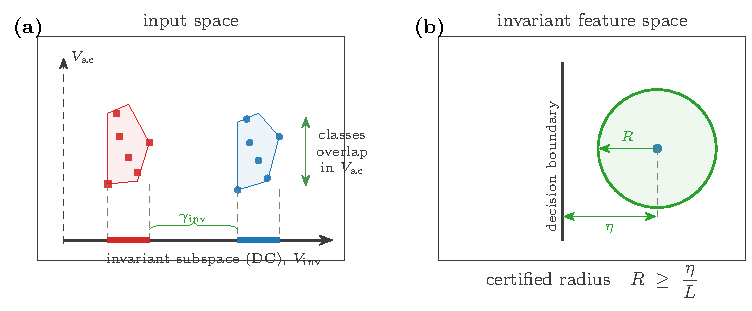
\includegraphics[width=\linewidth]{figures/concept.pdf}
\caption{The central criterion. \textbf{(a)} A shift-invariant linear classifier sees the data only through its projection onto the invariant subspace $\Vinv$ (the DC line for cyclic shift); the separation that remains is the invariant margin $\gamma_{\mathrm{inv}}$, the distance between the two projected class hulls (Theorem~\ref{thm:A}). Discriminative signal that lives in the orthogonal AC subspace $\Vac$ is invisible to invariance, where the classes overlap. \textbf{(b)} A margin $\eta$ in an invariant feature space certifies an $\ell_2$ robust radius $r_2\ge\eta/L$, with $L$ the Lipschitz constant of the invariant feature map $\Psi$ (\S\ref{sec:dich}); here $\eta=\gamma_{\mathrm{inv}}$ for the linear case. Invariance helps robustness only when the discriminative signal is preserved by the projection with positive margin.}
\label{fig:concept}
\end{figure}

\subsection{The exact invariant linear margin}
\begin{theorem}[Invariant linear margin equals projection separation]\label{thm:A}
A linear score $g(x)=w^\top x+b$ is shift-invariant for all $x$ if and only if $w\in\Vinv$, i.e.\ $w=c\mathbf 1$. Consequently, for any finite separable classes $X_+,X_-$, the invariant $\ell_2$ max-margin equals the separation of the DC-projected data,
\[
\gamma_{\mathrm{inv}}=\tfrac12\,\mathrm{dist}\big(I_+,I_-\big)
=\tfrac12\,\mathrm{dist}\big(\mathrm{conv}\,\Pi_{\mathrm{inv}}X_+,\ \mathrm{conv}\,\Pi_{\mathrm{inv}}X_-\big),
\]
where $I_\pm=\big[\min_{x\in X_\pm}\fdc(x),\ \max_{x\in X_\pm}\fdc(x)\big]$ are the intervals of DC values, with maximizing direction $\pm\mathbf 1/\sqrt\dd$ oriented toward the positive class. This holds for any finite separable dataset, not only the single-image case, and does not require orbit-closure.
\end{theorem}
\emph{Proof sketch.} Invariance forces $(S_{-s}w-w)^\top x=0$ for all $x,s$, hence $w\in\Vinv=\mathrm{span}(\mathbf 1)$ (only constant vectors are shift-fixed). With $w=c\mathbf 1$ the score depends on $x$ only through $\fdc(x)$, reducing the problem to one-dimensional thresholding of the DC values; the max-margin separator of two point sets on a line is the midpoint of the gap between their convex hulls (here the two intervals $I_\pm$), so the geometric margin is half the inter-interval distance. The one-sided form $\tfrac12(\min_{X_+}\fdc-\max_{X_-}\fdc)_+$ is the special case where $X_+$ lies above $X_-$ in DC coordinate. Full proof in Appendix~\ref{app:proofs}. \hfill$\square$

The single-image case, where each class is one image together with all its shifts, is the observation of \citet{ge2021shift} that a shift-invariant linear classifier separates classes only through their DC component. What Theorem~\ref{thm:A} adds is the exact convex-hull and interval form for an arbitrary finite separable dataset without orbit-closure, which is the form the architectural dissection of \S\ref{sec:exp} measures, together with the extension to any finite symmetry group below.

The same accounting holds for any finite symmetry group, with the DC projector replaced by the group-average projector.
\begin{proposition}[General finite-group invariant margin]\label{thm:finite-group}
Let a finite group $G$ act orthogonally on $\R^\dd$ by matrices $\{R_g\}$, with fixed subspace $V^G=\{v:R_gv=v\ \forall g\}$ and group-average projector $P_G=\tfrac1{|G|}\sum_{g\in G}R_g$, which is the orthogonal projector onto $V^G$. A linear score $w^\top x+b$ is exactly $G$-invariant if and only if $w\in V^G$, and the maximum invariant $\ell_2$ margin for finite separable classes is
\[
\gamma_{\mathrm{inv}}=\tfrac12\,\mathrm{dist}\big(\mathrm{conv}\,P_GX_+,\ \mathrm{conv}\,P_GX_-\big).
\]
Theorem~\ref{thm:A} is the cyclic case $P_G=\Pi_{\mathrm{inv}}$. (Proof in Appendix~\ref{app:proofs}.)
\end{proposition}

\subsection{The co-existence / trade-off dichotomy and the $\eta/L$ criterion}\label{sec:dich}
Theorem~\ref{thm:A} reduces ``does invariance hurt robustness?'' to ``is the discriminative signal preserved by projection onto the invariant subspace?''. If the projected classes overlap, $\gamma_{\mathrm{inv}}=0$ (forced trade-off); if they stay separated by $\eta>0$ with the invariant feature having Lipschitz constant $L$, the invariant classifier is simultaneously fully shift-consistent and robust with radius at least $\eta/L$. The governing scalar is therefore
\[
\boxed{\ \eta/L \;=\; \Sep_{\mathrm{inv}}/L\ } \qquad\text{(margin of the invariant feature, divided by its Lipschitz constant).}
\]
We stress $\eta/L$, not merely $\Sep_{\mathrm{inv}}>0$: invariance and robustness trade off whenever the margin that remains is small relative to its sensitivity, either because the projection discards the discriminative signal or because it is preserved only at a vanishing margin. The \citet{kamath2021canwehaveitall} construction is the first case (\S\ref{sec:recover}). The bound $r_2\ge\eta/L$ is a Lipschitz--margin certificate: there is no \emph{universal} converse, and the true robust radius can be arbitrarily larger than $\eta/L$ (for the invariant feature $t\mapsto t^{2n+1}$ on the DC line $t=\fdc(x)$, $\eta/L=1/(2n+1)$ while $r_2=1$, so the gap is unbounded). Under an explicit reachability condition, however, the certificate completes to a two-sided bracket.
\begin{proposition}[Two-sided bracket: a conditional converse]\label{prop:sandwich}
If the score is $L$-Lipschitz toward the boundary and admits a co-Lipschitz (lower-Lipschitz) constant $\alpha$ along a path reaching it, then $\eta/L\le r_2\le\eta/\alpha$ with condition number $\kappa:=L/\alpha\ge1$, so $\eta/L$ determines the robust radius up to $\kappa$. The bracket is exact ($r_2=\eta/\|w\|_2$, $\kappa=1$) for linear invariant features \citep{hein2017formal}; the $t^{2n+1}$ example above is the large-$\kappa$ regime, and for the power-spectrum surrogate both arms are explicit (verified numerically, realized $\kappa\approx1.6$--$2.4$). The certificate chain of \citet{tsuzuku2018lipschitz} (their Eq.~5) bounds $r_2$ only from below, through successively tighter Lipschitz constants; the upper bound $r_2\le\eta/\alpha$ is the matching arm that turns the one-sided certificate into a two-sided bracket. A tight converse of a different kind is already known for randomized smoothing, where \citet{cohen2019certified} show the smoothing radius is the largest the class probabilities alone can certify and is exact for linear bases; our bracket is instead deterministic and tied to a single fixed classifier, with looseness controlled by the explicit condition number $\kappa$ rather than by a worst case over classifiers. The full proof, with the explicit reaching-path and co-Lipschitz hypotheses, is in Appendix~\ref{app:bracket-lazy}.
\end{proposition}
We therefore read $\eta/L$ as a certificate and empirical predictor of robustness (\S\ref{sec:exp}) and, up to $\kappa$, as a characterization.

\paragraph{The excessive-invariance side.} The ratio $\eta/L$ lower-bounds model-score stability; a second quantity bounds whether the imposed invariance is semantically valid at the same radius. Let $y_\star$ be an oracle label and $g$ a $G$-invariant classifier correct at $x$, and define the orbit-flip radius $\rho_G(x)=\inf\{\|R_h x-x\|_2:\ y_\star(R_h x)\neq y_\star(x)\}$.
\begin{proposition}[Orbit-flip upper bound]\label{prop:rhoG}
If the set in the infimum is nonempty, the oracle-robust radius of $g$ at $x$ is at most $\rho_G(x)$: the orbit point $R_h x$ attaining it is correctly classified by $g$ yet wrong under the oracle, an invariance-based adversarial example. (Proof in Appendix~\ref{app:proofs}.)
\end{proposition}
A perturbation budget $\epsilon$ therefore admits a robust invariant classifier only if $\epsilon\le\eta/L$ (score stability) and $\epsilon<\rho_G$ (the imposed invariance does not cross the oracle boundary). This is the formal core of the excessive-invariance failure of \citet{tramer2020fundamental}: $\eta/L$ controls sensitivity-based attacks, $\rho_G$ controls invariance-based ones, and a model needs room under both.

\subsection{Nonlinear escape: a convolution-plus-pooling layer computes the power spectrum}
The invariant \emph{linear} family is one-dimensional (only $\fdc$). Nonlinear invariants are richer.
\begin{lemma}[Power-spectrum span]\label{lem:ps}
A circular-convolution layer with a quadratic activation and global average pooling computes, for filter $w$, $\;\Phi_{w}(x)=\tfrac1\dd\sum_s\big((w\star x)_s\big)^2=\tfrac1\dd\sum_k |\hat w_k|^2\,|\hat x_k|^2$. Varying a \emph{real} filter $w$ spans the nonredundant power coordinates $|\hat x_0|^2$, $|\hat x_{\dd/2}|^2$ (when $\dd$ is even), and the conjugate-pair sums $|\hat x_k|^2+|\hat x_{\dd-k}|^2$ for $0<k<\dd/2$; since $x$ is real these exhaust its power spectrum. (A complex filter isolates each individual $|\hat x_k|^2$.) These features are shift-invariant and supported on $\Vac$ for $k\neq0$.
\end{lemma}
\emph{Proof.} Cross-correlation has DFT $\overline{\hat w_k}\hat x_k$; Parseval with the unitary DFT gives the displayed identity. A real filter satisfies $|\hat w_k|^2=|\hat w_{\dd-k}|^2$, so it can weight a conjugate pair $\{k,\dd-k\}$ but not split it; concentrating it on one pair isolates $|\hat x_k|^2+|\hat x_{\dd-k}|^2$, while a complex filter supported on a single frequency isolates $|\hat x_k|^2$. \hfill$\square$

\begin{corollary}[Conditional robust radius]\label{cor:C}
For an invariant feature map $\Psi$ with achievable head margin $\eta=\tfrac12\,\mathrm{dist}(\mathrm{conv}\,\Psi(X_+),\mathrm{conv}\,\Psi(X_-))$ and Lipschitz constant $L$, the induced classifier has $\mathrm{SC}=1$ and $r_2\ge \eta/L$.
\end{corollary}
This is the standard Lipschitz-margin bound; its content is which $\Psi$ a shift-invariant architecture can realize (Lemma~\ref{lem:ps}), not the inequality itself, and as noted in \S\ref{sec:dich} it is a lower-bound certificate with no general converse. Here $\eta$ is the exact hard-margin separation of the feature sets. On a ball $\|x\|_2\le B$ the power-spectrum feature is $2B$-Lipschitz, which makes the certificate explicit, and Appendix~\ref{app:proofs} works out an exactly solvable two-subspace model whose every point has robust radius $a/\sqrt2$ under a quadratic invariant that no linear classifier can match. A complementary first-order fact: for the continuous shift generator, an invariant score has gradient orthogonal to the orbit tangent, so first-order perturbations along the continuous orbit do not change the score; the discrete shift is a finite secant and is not protected exactly.

\subsection{Recoveries and a corrected reconciliation}\label{sec:recover}
\textbf{\citet{ge2021shift}.} For the single white/black dot, $\fdc(\pm e_j)=\pm1/\sqrt\dd$, so Theorem~\ref{thm:A} gives $\gamma_{\mathrm{inv}}=1/\sqrt\dd$; in their one-sided convention the gap is $2/\sqrt\dd$ (their Corollary~1). The contrast ``unconstrained margin $1$ vs invariant $1/\sqrt\dd$'' is the two-image protocol: it compares the unshifted pair $\{e_j\},\{-e_j\}$ (unconstrained margin $1$) against the invariant classifier. On the orbit-closed dataset $\mathcal O(e_j)$ vs $\mathcal O(-e_j)$ the unconstrained linear max-margin is itself $1/\sqrt\dd$, so the gap is a property of that protocol, not of invariance alone. The power spectrum is sign-blind ($|\widehat{+e_j}_k|^2=|\widehat{-e_j}_k|^2$), so even the power-spectrum invariant cannot separate the dot, while the linear DC invariant separates it only at the weak margin $1/\sqrt\dd$: localized, phase-coded signal is the small-$\eta/L$ corner for both. A higher-order invariant escapes it, however: the bispectrum $\hat x_{k_1}\hat x_{k_2}\overline{\hat x_{k_1+k_2}}$ is also shift-invariant and separates $\pm e_j$ with margin $d^{-3/2}$ (it determines a generic signal up to shift), at the cost of a larger Lipschitz constant, hence a smaller certified $\eta/L$.

\textbf{\citet{kamath2021canwehaveitall}.} Their construction embeds the robustness--accuracy distribution of \citet{tsipras2019robustness} so that the discriminative signal is a binary cyclic code carried by the coordinates the shift \emph{permutes}, each with $\ell_\infty$ margin of order $1/\sqrt\dd$; the single coordinate the shift fixes carries only weak signal (correlation $p\ge\tfrac12$ with the label). A genuinely shift-invariant classifier can therefore use only that weak fixed coordinate and the power spectrum, and because the code is sign-coded its two classes have identical power spectra, so the invariant margin that remains is essentially zero. This is the same sign-blind, small-$\eta/L$ corner as the \citet{ge2021shift} dot, now embedded in a statistical model: the trade-off appears precisely because they take $p\to\tfrac12$, which empties the fixed coordinate. When $p$ is bounded away from $\tfrac12$, that coordinate is a strong invariant feature with $\Theta(1)$ margin and radius, which is our co-existence regime. So their impossibility is an instance of the $\eta/L$ criterion rather than a counterexample. We state this as an interpretation: a self-contained restatement of their exact distribution would be needed to make it a theorem in our framework.

\subsection{The margin--sensitivity coupling: \texorpdfstring{$\eta/L$}{eta/L} is a diagnostic, not a trainable target}\label{sec:coupling}
The certificate $r_2\ge\eta/L$ makes $\eta/L$ a target one might hope to train. We argue it is a diagnostic rather than a trainable objective, from three angles: an exact polar identity (Proposition~\ref{prop:split}) writes the gradient norm as the radial floor $M/\|x\|$ times a tangential factor, so the coupling is exactly characterized rather than an optimizer artifact; the ratio is scale-invariant, so its direct maximizer is degenerate (Lemma~\ref{lem:ratiodegen}); and four controlled interventions confirm that every attempt to lower or maximize it collapses the margin (Appendix~\ref{app:tmreg}). For a $k$-class score $f$ with true label $y$, write $M(x)=f_y(x)-\max_{j\neq y}f_j(x)$ for the signed logit margin and $\eta=\mathbb E[M]$, $L=\mathbb E\|\nabla M\|$ for its dataset means, the same $(\eta,L)$ the dissection of \S\ref{sec:exp} measures.

\begin{proposition}[Radial--tangential split of the margin gradient]\label{prop:split}
For a bias-free network with degree-one positively homogeneous activations (ReLU, leaky-ReLU, absolute value, maxout), $M$ is degree-one homogeneous. Writing $r=\|x\|_2$, $u=x/r$, and $m(u)=M(u)$, the input gradient splits into orthogonal radial and tangential parts,
\[
\nabla M(x)=m(u)\,u+\nabla_{\mathbb S}m(u),\qquad u\perp\nabla_{\mathbb S}m(u),
\]
so that
\[
\|\nabla M(x)\|_2=\frac{M(x)}{\|x\|_2}\sqrt{1+\bigl\|\nabla_{\mathbb S}\log m(u)\bigr\|_2^2}.
\]
The radial term is Euler's identity, $\langle\nabla M(x),x\rangle=M(x)$, which gives the floor $\|\nabla M(x)\|_2\ge M(x)/\|x\|_2$ and the cap $\eta/L\le\sup_i\|x_i\|_2$. The upper envelope $\|\nabla M(x_i)\|_2\le\tau\,M(x_i)/\|x_i\|_2$ holds exactly when the tangential factor is bounded, $\|\nabla_{\mathbb S}\log m(u_i)\|_2\le\sqrt{\tau^2-1}$; equivalently $\tau_i=\sec\angle(\nabla M(x_i),x_i)$. This $\tau$ is the slack between the gradient and its radial floor, distinct from the bracket condition number $\kappa=L/\alpha$ of Proposition~\ref{prop:sandwich} (the certificate's looseness): $\tau=1$ means the gradient is purely radial, $\kappa=1$ means the certificate $r_2=\eta/L$ is tight. (Proof in Appendix~\ref{app:proofs}.)
\end{proposition}

The tangential factor is not controlled by homogeneity, which fixes only the radial part; it is set by the data geometry of the trained solution. For a linear classifier $g(x)=w^\top x$ at its hard-margin solution the factor is exact, $\tau_i=\|x_i\|_2/\gamma$ with $\gamma$ the geometric margin \citep{soudry2018implicit}, and sharp. For a bias-free homogeneous network the same data condition number bounds it, $\tau_i\le B_i\|x_i\|_2/\gamma_{\mathrm{IB}}$ (with $B_i=\sqrt2$ for a depth-$D$ ReLU network under the product-of-spectral-norms complexity), where $\gamma_{\mathrm{IB}}$ is the normalized margin the gradient-descent solution actually achieves (Appendix~\ref{app:envelope}); no universal constant exists, since a four-point construction already forces $\tau\to\infty$. The achieved margin is the honest denominator: gradient descent on homogeneous networks converges to a KKT point of the max-margin program \citep{lyu2020gradient,ji2020directional}, which for ReLU networks need not be globally max-margin \citep{vardi2022margin}, so the bound cannot use the global margin but does hold with $\gamma_{\mathrm{IB}}$, recovering the global form when the two coincide. The envelope is therefore a property of the solution's data geometry, not a trainable law. Empirically the factor is large, with $\|\nabla M\|_2$ exceeding the radial floor $M/\|x\|_2$ by roughly $26$ on the trained networks (Figure~\ref{fig:coupling-split}); this is exactly the slack that lets a gradient penalty lower $\|\nabla M\|$ at the diagnostic level while the margin falls with it, so $\eta/L$ diagnoses robustness but is not itself a target.

\begin{figure}[t]\centering

\includegraphics[width=\linewidth]{figures/coupling_split.pdf}
\caption{The margin gradient of a homogeneous network splits exactly into a radial part fixed by Euler's identity and a free tangential part (Proposition~\ref{prop:split}). \emph{Left:} at a data point $x$ with direction $u=x/\|x\|$, $\nabla M(x)=m(u)\,u+\nabla_{\mathbb S}m(u)$; the radial component equals the Euler floor $M(x)/\|x\|$ while the tangential component $\nabla_{\mathbb S}m(u)$ is unconstrained, and the angle $\theta$ between $\nabla M$ and $x$ sets $\|\nabla M\|=(M/\|x\|)\sec\theta$. \emph{Right:} the envelope factor $\tau=\|\nabla M\|/(M/\|x\|)=\sqrt{1+\|\nabla_{\mathbb S}\log m(u)\|^2}$ measures how far the gradient exceeds its radial floor. It equals $1$ only when $\nabla M$ is purely radial ($\nabla_{\mathbb S}\log m=0$); for a linear or exactly invariant score it is the data condition number $\|x\|/\gamma$, and at the trained networks it is large ($\tau\approx26$), the slack that makes $\eta/L$ a diagnostic rather than a trainable target. ($\tau$ is the gradient-floor slack, distinct from the bracket condition number $\kappa=L/\alpha$ of Proposition~\ref{prop:sandwich}.)}
\label{fig:coupling-split}
\end{figure}

A further degeneracy rules out the obvious workaround of maximizing the ratio directly.
\begin{lemma}[Scale-invariance of the ratio]\label{lem:ratiodegen}
The per-sample ratio $M(x)/\|\nabla M(x)\|$ is invariant to positive rescaling of the score, $f\mapsto cf$ for $c>0$, since numerator and denominator scale together. Hence an objective that maximizes $\eta/L$ (equivalently, penalizes $\|\nabla M\|/M$ over correctly classified points) is blind to the absolute margin and admits the constant classifier $\nabla M\equiv0$ as a global optimizer, so maximizing $\eta/L$ directly is ill-posed as a training objective. (Proof in Appendix~\ref{app:proofs}.)
\end{lemma}

Together, Proposition~\ref{prop:split} and Lemma~\ref{lem:ratiodegen} explain why first-order training of $\eta/L$ does not help: maximizing the ratio is degenerate, and at fixed architecture the certificate is tight only up to the tangential factor the operating point already sets, so lowering $\|\nabla M\|$ trades against the margin. Appendix~\ref{app:tmreg} confirms this with four controlled interventions, all of which collapse the margin.

\section{Optimization: does gradient descent reach the robust invariant solution?}\label{sec:opt}
The structural theory says robust shift-invariant classifiers exist; it does not say gradient descent finds them. For unconstrained two-layer ReLU networks on near-orthogonal cluster data, the implicit bias of gradient descent provably selects a non-robust max-margin solution even though robust ones exist \citep{vardi2022gradient,frei2023double}, via \emph{feature averaging} \citep{li2025feature}; \citet{min2024can} conjecture that changing the architecture re-points this bias, and a natural hope is that hard-wired shift-invariance is such a lever. Testing that hope needs orbit-structured data on which the non-robustness premise genuinely holds. We characterize exactly when it can, via the rank of an orbit, and find that the two canonical orbit constructions both fail to, in opposite ways.

\begin{lemma}[Orbit-bundle form]\label{lem:bundle}
A circular-convolution-plus-global-pooling network equals a two-layer network whose neurons are tied into shift-orbit bundles (one filter spawns all $\dd$ of its shifts, sharing one output weight) and whose feature is an orbit average. (Exact; structural.)
\end{lemma}

\begin{lemma}[Rank of a shift orbit]\label{lem:rank}
For a base pattern $u\in\R^\dd$, the cyclic orbit $\{S_s u\}_{s\in\Z_\dd}$ has rank exactly $\#\{k:\hat u_k\neq0\}$, the number of nonzero Fourier coefficients of $u$.
\end{lemma}
\emph{Proof.} The matrix of orbit columns is circulant, hence diagonalized by the DFT with eigenvalues $\propto\hat u_k$; the rank is the number of nonzero eigenvalues. \hfill$\square$

\begin{proposition}[The canonical orbit bases are degenerate, in opposite ways]\label{prop:rank}
Let each class be the shift orbit of a single base pattern. (i) For a single cosine of frequency $k$, Lemma~\ref{lem:rank} gives orbit rank $2$ (it spans $\{\cos,\sin\}$ at frequency $k$), violating the near-orthogonal $\Omega(\dd)$-cluster assumption of \citet{frei2023double,li2025feature}; moreover the signed orbit mean, the direction that carries the non-robustness conclusion in those works, is $\mathbf 0$. (ii) For a localized spike $e_j$, the orbit is full-rank and orthonormal (the cluster assumption holds) but the power spectrum is phase-blind, so $\Sep(\Psi)=0$ and the invariant nonlinear classifier cannot separate the two classes. Thus neither canonical base is a valid testbed for the re-pointing hope: in (i) the non-robustness premise fails, in (ii) the invariant-separation conclusion fails.
\end{proposition}
\emph{Verification.} For $\dd=64$, $k=5$: the cosine orbit has numerical rank $2$ and signed mean of norm $1.7\times10^{-16}$; the spike orbit has rank $\dd$ and power-spectrum gap $0$. \hfill$\square$

\begin{proposition}[The degeneracy is non-generic]\label{prop:generic}
If a base $u$ has all Fourier coefficients nonzero, its orbit is full-rank (Lemma~\ref{lem:rank}); and two such bases with distinct power spectra are power-spectrum separable. Hence generic single-orbit data is simultaneously full-rank and invariant-separable, so the degenerate corner of Proposition~\ref{prop:rank} does not cover single-orbit data in general.
\end{proposition}

Lemma~\ref{lem:rank} and Propositions~\ref{prop:rank}--\ref{prop:generic} are modest structural contributions: they pin down exactly which orbit data is degenerate and show the two textbook constructions are the degenerate cases (which explains why an unconstrained network is already competitive on them), while generic single-orbit data is not degenerate. They do \emph{not} close the optimization gap, but a direct test on synthetic orbit data sharpens it. Training unconstrained versus weight-tied shift-invariant ReLU networks on the same orbit data shows the effect is \emph{data-model-dependent}. On generic orbit data, shift-invariance is provably \emph{margin-free}: on orbit-closed data the invariant and unconstrained two-layer-ReLU max-margin values coincide (Corollary~\ref{cor:no-gap-var}), because orbit-averaging an unconstrained solution gives an invariant one of equal minimum norm; so weight sharing cannot raise the margin there, and indeed the unconstrained network self-symmetrizes with no feature-averaging collapse. Here ``max-margin'' is the directional limit gradient descent reaches on homogeneous networks \citep{soudry2018implicit,lyu2020gradient,ji2020directional}. But on near-orthogonal cluster-geometry data the invariant architecture reaches a substantially larger $\eta/L$ than the unconstrained one (a factor $1.2$ in the rich regime, up to $\sim$$4.5$ in the lazy regime, robust across $4$--$8$ orbits and $d\in\{64,128\}$), at equal margin, so the larger realized $\eta/L$ comes through a smaller Lipschitz constant, and it is largest exactly where the unconstrained network fails to self-symmetrize. So whether invariance re-points the implicit bias toward robustness depends on the data geometry. In the lazy/NTK regime orbit-averaging is the orthogonal projection onto the invariant subspace of the tangent RKHS \citep{elesedy2021provably}, so the invariant minimum-norm problem is never harder than the unconstrained one. On orbit-complete data, however, the unconstrained minimum-norm interpolant is \emph{itself} already invariant, because Reynolds averaging preserves the orbit-constant margin constraints and the RKHS norm is strictly convex; the two minimum-norm certified Lipschitz constants therefore \emph{coincide} rather than differ (Theorem~\ref{thm:lazy-cluster}, Appendix~\ref{app:bracket-lazy}). The observed cluster-geometry advantage is consequently a property of the \emph{realized} finite-width solution (its local $\eta/L$), not of a smaller minimum-norm certificate. The rich (small-init) regime and the bare-ReLU trajectory remain open, on the same wall reached by \citet{frei2023double,min2024can,li2025feature}. Empirically (\S\ref{sec:exp}), $\eta/L$ predicts the robustness of trained models regardless.

\section{Experiments}\label{sec:exp}
Code, training configurations, trained checkpoints, and the per-cell results behind every correlation below are provided with the submission, so each reported number is reproducible end to end.

\paragraph{Structural predictions, training-free (confirmed).} We compute, per dataset, the unconstrained linear margin $\Sep(\mathrm{Id})$, the invariant linear margin $\Sep(\Pi_{\mathrm{inv}})$ (Theorem~\ref{thm:A}), and the power-spectrum margin via a hard-margin SVM (Table~\ref{tab:struct}). The single dot is separable by an unconstrained classifier (margin $1$), only weakly by linear invariance ($1/\sqrt\dd$), and not at all by the power spectrum (sign-blind). The orthogonal-frequency data of \citet{ge2021shift} (each class the span of odd, resp.\ even, frequencies) is separable by \emph{neither} linear classifier yet separable by the power-spectrum invariant: invariance helps through the right nonlinear feature.

\begin{table}[h]\centering
\caption{Achievable separation by classifier family (training-free), $\dd=64$ so $1/\sqrt\dd=0.125$.}
\label{tab:struct}
\begin{tabular}{lcccc}
\toprule
dataset & $\Sep(\mathrm{Id})$ & $\Sep(\Pi_{\mathrm{inv}})$ & $\eta_{\Psi}$ (power spec.) & $\eta_\Psi/L$ \\
\midrule
dot ($+e_0/-e_0$) & $1.000$ & $0.125$ & $0.000$ & $0$ \\
frequency, single & $0.000$ & $0.000$ & $361.9$ & $3.10$ \\
frequency, spans (Ge) & $0.000$ & $0.000$ & $5.75$ & $0.378$ \\
\bottomrule
\end{tabular}
\end{table}

\paragraph{Architectural dissection ($\eta/L$ predicts robustness; shift-consistency does not).} We train seven architectures (a fully connected baseline; a single convolution-plus-global-pooling shift-invariant model; multi-layer convolutions with max/average pooling and an optional dense layer), each with and without batch-normalization where applicable, on $16{,}000$ images for $25$ epochs, three seeds, on GPU, for both MNIST and Fashion-MNIST. As the dataset-comparable robustness measure we use the per-sample \emph{robust radius} $r_2$ (the smallest $\ell_2$-PGD perturbation that flips the label), of which $\eta/L$ is a lower bound; fixed-$\epsilon$ robust accuracy is misleading across datasets because of floor effects. Table~\ref{tab:diss} reports the MNIST per-model means. Across the seven configurations, $\eta/L$ predicts the robust radius with Spearman $\rho=+0.96$ on MNIST and $+0.71$ on Fashion-MNIST, whereas shift-consistency predicts it on neither ($\rho=-0.31$ and $0.00$). The single shift-invariant model has consistency $1.0$ yet the smallest robust radius, the sharpest illustration that consistency does not imply robustness. Batch-normalization raises clean accuracy and lowers fixed-$\epsilon$ robust accuracy in both the fully connected and convolutional pairs, consistent with \citet{galloway2019batchnorm}; under the per-sample robust radius, however, the change reverses sign and is small, which is precisely why we treat the radius, not fixed-$\epsilon$ accuracy, as the dataset-comparable measure.

\begin{table}[h]\centering
\caption{MNIST dissection (means over 3 seeds, $n{=}16{,}000$, 25 epochs). Primary metric: per-sample $\ell_2$ robust radius $r_2$ (smallest label-flipping $\ell_2$-PGD perturbation), of which $\eta/L$ is a lower bound. Fixed-$\epsilon$ robust accuracy (rob$_\epsilon$, $\ell_2$ at $\epsilon{=}1.5$) is shown for comparison.}
\label{tab:diss}
\footnotesize
\begin{tabular}{lrccccc}
\toprule
model & params & clean & consist. & $r_2$ & rob$_\epsilon\,\ell_2$ & $\eta/L$ \\
\midrule
FC (depth 2)            & 269k & 0.971 & 0.281 & 0.938 & 0.060 & 0.592 \\
FC (depth 2) + BN       & 270k & 0.973 & 0.292 & 0.962 & 0.043 & 0.668 \\
conv d1 k5 GAP          & 4.6k & 0.569 & 1.000 & 0.457 & 0.047 & 0.376 \\
conv d1 k5 GAP + BN     & 4.9k & 0.647 & 1.000 & 0.486 & 0.022 & 0.557 \\
conv d2 k3 max          & 212k & 0.987 & 0.473 & 1.846 & 0.477 & 1.443 \\
conv d2 k3 avg          & 212k & 0.984 & 0.475 & 1.658 & 0.399 & 1.537 \\
conv d2 k3 max + dense  & 953k & 0.986 & 0.487 & 1.944 & 0.570 & 1.627 \\
\midrule
\multicolumn{7}{l}{Spearman over 7 rows: $\eta/L$ vs $r_2 = +0.96$ (MNIST), $+0.71$ (Fashion); consist.\ vs $r_2 = -0.31$, $0.00$.}\\
\bottomrule
\end{tabular}
\end{table}

\paragraph{Capacity-matched CIFAR-10 dissection.} We repeat the test on CIFAR-10 with a controlled comparison along the shift-invariance axis at matched capacity. Four architectures share one channel schedule, hence an identical parameter count, and differ only in the shift-invariance operator: a \emph{standard} network (max-pooling, zero padding); an \emph{anti-aliased} network with blur-pooled downsampling \citep{zhang2019making}; an \emph{exact cyclic} network (circular padding, global pooling, no spatial subsampling) that is exactly invariant to integer circular shifts; and a \emph{shift-augmented} network, the standard architecture trained with random circular shifts so its invariance is learned rather than built in. We train three seeds at two widths and report clean accuracy, circular-shift consistency, the per-sample $\ell_2$ robust radius $r_2$ from the decoupled direction and norm (DDN) minimum-norm attack \citep{rony2019decoupling} (validated against the closed-form radius of a linear model to under one percent), and the active logit margin $M$ (the gap between the correct-class logit and the highest other logit), summarized by its mean $\eta=\mathbb{E}[M]$ and mean input-gradient norm $L=\mathbb{E}\|\nabla M\|_2$ (Table~\ref{tab:cifar}). The threat-matched ratio $\eta/\|\nabla M\|_q$ used under adversarial training takes $q$ the dual norm of the attack. Clean accuracy is comparable across arms, with the exactly invariant model slightly lower. AutoAttack \citep{croce2020reliable} at the standard CIFAR thresholds drives every model to zero robust accuracy, as expected for models that are not adversarially trained; this floor is the reason we use the per-sample radius as the comparable quantity. At smaller $\ell_2$ radii where AutoAttack is informative, the radius and AutoAttack agree: across arms the fraction of points with $r_2>\epsilon$ matches AutoAttack robust accuracy at $\epsilon\in\{0.05,0.10,0.15,0.25\}$ to a mean absolute gap of $0.014$ (maximum $0.025$), so the radius is not inflated by gradient masking.

\begin{table}[h]\centering
\caption{Capacity-matched CIFAR-10 dissection (means over 3 seeds). All four arms have identical parameter counts at each width ($288.7$k at $w{=}32$, $1.15$M at $w{=}64$). $r_2$ is the per-sample $\ell_2$ robust radius (DDN, on correctly classified points); $\eta$ and $L$ are the mean active logit margin and its mean input-gradient norm. AutoAttack at $\ell_\infty{=}8/255$ and $\ell_2{=}0.5$ is $0.000$ for every arm (the floor that motivates $r_2$).}
\label{tab:cifar}
\footnotesize
\begin{tabular}{llcccccc}
\toprule
arm & $w$ & clean & consist. & $r_2$ & $\eta$ & $L$ & $\eta/L$ \\
\midrule
standard      & 32 & 0.888 & 0.854 & 0.099 & 7.85 & 81.9 & 0.096 \\
anti-aliased  & 32 & 0.900 & 0.887 & 0.116 & 7.75 & 66.4 & 0.117 \\
exact cyclic  & 32 & 0.871 & 1.000 & 0.080 & 5.06 & 64.5 & 0.079 \\
shift-aug     & 32 & 0.903 & 0.928 & 0.106 & 6.99 & 67.2 & 0.104 \\
\midrule
standard      & 64 & 0.912 & 0.891 & 0.119 & 8.34 & 71.3 & 0.117 \\
anti-aliased  & 64 & 0.919 & 0.909 & 0.141 & 8.57 & 59.4 & 0.144 \\
exact cyclic  & 64 & 0.897 & 1.000 & 0.090 & 6.42 & 73.0 & 0.088 \\
shift-aug     & 64 & 0.921 & 0.943 & 0.117 & 8.75 & 75.1 & 0.117 \\
\bottomrule
\end{tabular}
\end{table}

\begin{figure}[h]\centering

\includegraphics[width=\linewidth]{figures/cifar_etaL_vs_radius.pdf}
\caption{CIFAR-10, eight capacity-matched architecture-by-width cells (bold markers) and their three seeds (faint). Left: $\eta/L$ tracks the $\ell_2$ robust radius (Pearson $0.998$, Spearman $0.98$; $0.997$ across individual seeds). Right: shift-consistency does not predict it; the exactly invariant model (red) has consistency $1.0$ and the smallest radius.}
\label{fig:cifar-pred}
\end{figure}

\begin{figure}[h]\centering

\includegraphics[width=\linewidth]{figures/cifar_decomposition.pdf}
\caption{Margin/Lipschitz decomposition of the robust-radius change relative to the standard baseline, at each width ($\Delta\log(\eta/L)=\Delta\log\eta-\Delta\log L$; higher is more robust). Anti-aliasing raises $\eta/L$ by lowering the Lipschitz constant with the margin roughly unchanged; exact cyclic invariance lowers $\eta/L$ by shrinking the margin.}
\label{fig:cifar-decomp}
\end{figure}

The CIFAR-10 dissection makes two points. First, $\eta/L$ predicts the robust radius across all eight capacity-matched cells (Pearson $0.998$, Figure~\ref{fig:cifar-pred}), while shift-consistency does not: the exactly invariant model has perfect consistency yet the smallest radius, the clearest separation of the two. Second, the decomposition shows the two robustness-changing operators act through different terms (Figure~\ref{fig:cifar-decomp}). Because the arms are capacity-matched and trained with the identical loss, their logit gauge is comparable, so the per-term split $\Delta\log(\eta/L)=\Delta\log\eta-\Delta\log L$ is read at that fixed gauge. Anti-aliasing leaves the margin essentially unchanged and lowers the Lipschitz constant ($\Delta\log L\approx-0.2$), gaining robustness through reduced input sensitivity. Exact cyclic invariance instead shrinks the margin ($\Delta\log\eta\approx-0.26$ to $-0.44$) and loses robustness, the real-data form of the \citet{ge2021shift} collapse: forcing invariance costs discriminative margin even while it makes the model perfectly shift-consistent. This is the structural criterion of \S\ref{sec:dich} made operational: invariance helps robustness only when it does not cost margin.

\paragraph{Under adversarial training.} To test whether the picture holds under a strong standardized attack, we PGD-adversarially train \citep{madry2018towards} the same four arms ($\ell_\infty$, $\epsilon=8/255$, $7$ steps; two widths, two seeds) and evaluate with AutoAttack at the RobustBench thresholds (Table~\ref{tab:cifar-at}). Adversarial training makes AutoAttack informative: robust accuracy is now $26$--$42\%$ at $\ell_\infty=8/255$, with no gradient masking (AutoAttack stays below matched PGD for every arm). Three things hold. (i) Shift-consistency remains strongly \emph{anti}-correlated with robustness (Pearson $-0.88$ against AutoAttack); the exactly invariant model has consistency $1.0$ and the lowest robust accuracy of the four. (ii) The $\eta/L$ criterion still predicts robustness once its norm is matched to the threat: the $\ell_\infty$-matched ratio $\eta/\|\nabla M\|_1$, using the dual norm of the $\ell_\infty$ attack, tracks AutoAttack robust accuracy with Pearson $0.88$ (Figure~\ref{fig:cifar-at}), whereas the $\ell_2$ ratio ($0.55$) and the $\ell_2$ robust radius (near zero) do not, because adversarial training increases robustness in $\ell_\infty$, not $\ell_2$. (iii) The robustness ordering is anti-aliased $\ge$ standard $\approx$ shift-augmented $>$ exact cyclic, the same direction as standard training. One confound deserves attention: the exactly invariant arm reaches lower clean accuracy under adversarial training ($0.57$--$0.63$ vs.\ $0.69$--$0.78$), so with only four arms one could read its robustness deficit as reduced fitting rather than margin geometry. The ResNet-scale dissection below settles this directly: its added low-invariance arms carry the anti-prediction across six arms spanning the full consistency range, not the single exactly invariant outlier, and it survives controlling for clean accuracy. The threat-matched $\eta/L$ law is likewise not a clean-accuracy artifact.

\begin{table}[h]\centering
\caption{PGD-adversarially trained CIFAR-10 dissection (means over 2 seeds; $\ell_\infty$ training at $\epsilon=8/255$). AA$_\infty$ and AA$_2$ are AutoAttack robust accuracy at $\ell_\infty{=}8/255$ and $\ell_2{=}0.5$; $\eta/\|\nabla M\|_1$ is the $\ell_\infty$-matched margin-to-sensitivity ratio. Parameter counts per width are identical to Table~\ref{tab:cifar}.}
\label{tab:cifar-at}
\footnotesize
\begin{tabular}{llcccccc}
\toprule
arm & $w$ & clean & consist. & AA$_\infty$ & AA$_2$ & $\eta/\|\nabla M\|_1$ & $\eta/L_2$ \\
\midrule
standard      & 32 & 0.712 & 0.794 & 0.375 & 0.531 & 0.0420 & 1.190 \\
anti-aliased  & 32 & 0.724 & 0.802 & 0.388 & 0.540 & 0.0429 & 1.191 \\
exact cyclic  & 32 & 0.569 & 1.000 & 0.261 & 0.402 & 0.0371 & 1.104 \\
shift-aug     & 32 & 0.694 & 0.867 & 0.359 & 0.503 & 0.0417 & 1.149 \\
\midrule
standard      & 64 & 0.766 & 0.820 & 0.408 & 0.567 & 0.0411 & 1.133 \\
anti-aliased  & 64 & 0.775 & 0.823 & 0.419 & 0.577 & 0.0423 & 1.154 \\
exact cyclic  & 64 & 0.633 & 1.000 & 0.294 & 0.449 & 0.0365 & 1.080 \\
shift-aug     & 64 & 0.750 & 0.891 & 0.395 & 0.548 & 0.0409 & 1.100 \\
\bottomrule
\end{tabular}
\end{table}

\begin{figure}[h]\centering

\includegraphics[width=\linewidth]{figures/cifar_at_predict.pdf}
\caption{PGD-adversarially trained CIFAR-10 (eight cells, bold; two seeds, faint). Left: the $\ell_\infty$-matched ratio $\eta/\|\nabla M\|_1$ tracks AutoAttack robust accuracy at $\ell_\infty=8/255$ (Pearson $0.88$). Right: shift-consistency anti-predicts it (Pearson $-0.88$); the exactly invariant model (red) has consistency $1.0$ and the lowest robust accuracy.}
\label{fig:cifar-at}
\end{figure}

\paragraph{Generality across datasets and threats.} The two laws hold when we repeat the adversarial-training dissection on MNIST and Fashion-MNIST ($\ell_\infty$) and on CIFAR-10 under an $\ell_2$ threat (Table~\ref{tab:at-general}; the per-arm robust accuracies behind these correlations are in Appendix~\ref{app:at-tables}). Across all four conditions the threat-matched ratio $\eta/\|\nabla M\|_q$ (with $q$ the dual norm of the attack) predicts AutoAttack robust accuracy (up to $+0.92$), exceeding the mismatched ratio in every $\ell_\infty$ condition, and shift-consistency \emph{anti}-predicts it (Pearson $-0.44$ to $-0.92$). The anti-prediction is weakest on MNIST: at $\ell_\infty{=}0.3$ every arm is roughly $94\%$ robust, so the AutoAttack spread across arms is narrow and the consistency correlation, while still negative, is not significant at this grid size; the threat-matched $\eta/L$ stays a strong predictor there ($+0.92$) because it does not saturate. The one place the matched ratio does not lead is $\ell_2$-CIFAR, where the two are comparable and the mismatched ratio is in fact marginally higher (matched $+0.88$, mismatched $+0.91$) because the $\ell_1$ and $\ell_2$ gradient norms run nearly proportional there; the threat-matching is then better read at the metric level, where the $\ell_2$ robust radius predicts $\ell_2$ AutoAttack ($+0.80$) even though it had decoupled under $\ell_\infty$ training. No gradient masking appears in any condition (AutoAttack $\le$ matched PGD throughout), and the exact-cyclic arm has the lowest robust accuracy in every condition, again through a margin deficit ($\Delta\log\eta<0$ for circular on all datasets).

\begin{table}[h]\centering
\caption{Adversarial-training dissection across datasets and threat models (four arms $\times$ two widths $\times$ two seeds; Pearson computed over the eight $(\mathrm{arm},\mathrm{width})$ cell means against AutoAttack robust accuracy at the threat threshold). Matched ${=}$ dual norm of the training threat ($\ell_1$ gradient for $\ell_\infty$, $\ell_2$ gradient for $\ell_2$). The consistency anti-prediction and threat-matched $\eta/L$ prediction hold throughout.}
\label{tab:at-general}
\footnotesize
\begin{tabular}{llccc}
\toprule
dataset & threat & consist.\ vs AA & matched $\eta/\|\nabla M\|_q$ & mismatched \\
\midrule
CIFAR-10      & $\ell_\infty\ 8/255$ & $-0.88$ & $+0.88$ & $+0.55$ \\
CIFAR-10      & $\ell_2\ 0.5$        & $-0.81$ & $+0.88$ & $+0.91$ \\
MNIST         & $\ell_\infty\ 0.3$   & $-0.44$ & $+0.92$ & $+0.90$ \\
Fashion-MNIST & $\ell_\infty\ 0.1$   & $-0.92$ & $+0.71$ & $+0.68$ \\
\bottomrule
\end{tabular}
\end{table}

\paragraph{Statistical power.} Because each condition above has eight cells, we repeat the CIFAR-10 dissection on denser grids and report bootstrap $95\%$ confidence intervals (resampling cells) with a two-sided permutation test. On a $24$-cell standard-training grid (six widths, four seeds), shift-consistency is not a significant predictor of the robust radius (Pearson $-0.33$, CI $[-0.68,+0.09]$, $p=0.11$), consistent with the near-zero MNIST and Fashion-MNIST values, whereas $\eta/L$ predicts it almost exactly ($+0.998$, CI $[+0.997,+0.999]$, $p<10^{-3}$). The $\eta/L$--radius value is high by construction: $\eta/L$ is a first-order lower bound on $r_2$ and these models are close to locally linear, so this correlation is the across-cell face of the per-sample certificate (\S\ref{sec:exp}) rather than a separate finding. The load-bearing result is the dissociation, that the architectural axis summarized by shift-consistency carries no information about the radius while the margin-to-sensitivity axis carries almost all of it. On a $12$-cell adversarially trained grid (three widths, three seeds) the anti-prediction is significant: shift-consistency versus AutoAttack is $-0.75$ (CI $[-0.92,-0.02]$, $p=0.006$) and the threat-matched ratio is $+0.83$ (CI $[+0.49,+0.93]$, $p=0.002$), with the mismatched ratio not significant ($+0.27$, $p=0.39$) and no gradient masking. The strong consistency anti-prediction is thus specific to adversarial training.

\paragraph{Scaling to a ResNet backbone.} To check that the dissection is not an artifact of small networks, we repeat it on a PreActResNet-18 backbone on CIFAR-10 and CIFAR-100. We keep the four capacity-matched arms and add two parameter-matched low-invariance arms (a zero-padding variant and an explicitly aliased max-pool variant) at two widths and up to three seeds; here the exactly invariant arm uses adaptive polyphase sampling \citep{chaman2021truly} rather than circular padding, so the exact-invariance result is reproduced through a second mechanism. All arms are PGD-adversarially trained at $\ell_\infty{=}8/255$ with best-robust early stopping \citep{rice2020overfitting} and evaluated with AutoAttack (Figure~\ref{fig:resnet-at}). Both laws carry over at scale. Over the twelve architecture-by-width cells the threat-matched ratio $\eta/\|\nabla M\|_1$ predicts AutoAttack robust accuracy with Pearson $+0.91$ ($p<10^{-3}$; $+0.77$ over the twenty-four individual trained models with a cell-resampling bootstrap), and under standard training $\eta/L$ predicts the $\ell_2$ robust radius with Pearson $+0.96$; shift-consistency anti-predicts robust accuracy with Pearson $-0.81$ ($p=0.002$), and this persists when we control for clean accuracy (partial correlation $-0.82$). Across the four capacity-matched arms alone the anti-prediction is weak and not significant ($-0.43$); it sharpens to $-0.81$ only once the two low-invariance arms widen the consistency range. This is the point rather than a caveat: shift-consistency relates to robustness only across a broad enough span of the invariance axis and, even then, more weakly and with the opposite sign to what the anti-aliasing reading would suggest, whereas the threat-matched $\eta/L$ predicts robustness throughout. No gradient masking appears (AutoAttack stays below matched PGD for every cell, including the non-differentiable adaptive-polyphase arm). On CIFAR-100 the threat-matched law holds in the same direction (Spearman $+1.0$ over the four arms), underpowered at four cells.

Why shift-consistency is the unreliable signal is visible in the consistency axis itself: a ResNet backbone is already strongly shift-invariant, so over the four capacity-matched arms consistency is squeezed into $[0.93,1.00]$ and stops discriminating, and only once the two low-invariance arms widen it to $[0.86,1.00]$ does the anti-prediction reappear. The margin-to-Lipschitz ratio does not saturate this way and separates the arms throughout, so on a strong backbone shift-consistency is nearly constant while $\eta/L$ still tracks robustness.

\begin{figure}[t]\centering

\includegraphics[width=\linewidth]{figures/resnet_at_predict_cifar10.pdf}
\caption{PGD-adversarially trained PreActResNet-18 on CIFAR-10 (twelve architecture-by-width cells, bold; seeds, faint). Left: the $\ell_\infty$-matched ratio $\eta/\|\nabla M\|_1$ tracks AutoAttack robust accuracy at $\ell_\infty{=}8/255$ (Pearson $+0.91$). Right: shift-consistency anti-predicts it (Pearson $-0.81$); the exactly invariant adaptive-polyphase arm (red) has consistency $1.0$ and the lowest robust accuracy, while the low-invariance arms (gray, purple) sit at low consistency and high robustness.}
\label{fig:resnet-at}
\end{figure}

\paragraph{A graded anti-aliasing control at matched clean accuracy.} The arms compared so far also differ in how well they fit, so we add a controlled sweep that varies anti-aliasing strength while holding clean accuracy fixed. We PGD-adversarially train the same backbone with blur-pool filters of increasing width (Rect-2, Tri-3, Bin-5, Bin-7), which raise shift-invariance at nearly constant clean accuracy, together with the standard (aliased) and exact-cyclic endpoints (six arms, two widths, five seeds; Figure~\ref{fig:graded}). Three things follow. First, across the anti-aliasing family clean accuracy is matched within each width-and-seed cell to about one point (range $0.010$), yet robust accuracy rises ($0.390\to0.404$): the anti-aliasing arms beat the aliased baseline in $39$ of $40$ cells (paired gain $+0.013$, bootstrap $95\%$ CI $[+0.011,+0.014]$; the strongest, Bin-5, beats standard by $+0.015$, paired $t$-test $p<0.001$), and the gain tracks a paired margin gain ($\eta:+0.062$, positive in every cell) at a roughly constant Lipschitz term. At matched fitting, anti-aliasing buys robustness through the margin, the opposite term to the one it acts on under standard training (where it instead lowers the Lipschitz constant, Figure~\ref{fig:cifar-decomp}). So invariance can help, and here it does so with no clean-accuracy cost. Second, shift-consistency is non-monotonic in robustness: it is nearly flat ($\approx0.80$) across the anti-aliasing family and then jumps to $1.0$ at the exact-cyclic arm, which is the \emph{least} robust of the six, so higher consistency does not imply higher robust accuracy, whereas the threat-matched $\eta/L$ orders the arms by robustness (Pearson $+0.93$). Third, and we state this plainly, the exact-cyclic arm's robustness deficit cannot be separated from a clean-accuracy deficit: forcing exact invariance collapses the margin ($\eta:1.53\to0.85$), and that one collapse lowers clean accuracy ($0.73\to0.58$) and robust accuracy together, so across the six arms clean accuracy predicts robustness as strongly as $\eta/L$ does. The right reading is therefore not that clean accuracy is a confounder to be removed, but that the margin is the upstream quantity both depend on: $\eta/L$ tracks robustness because it is built on the margin the invariance operator changes, while shift-consistency, which ignores the margin, does not.

\begin{figure}[t]\centering

\includegraphics[width=0.92\linewidth]{figures/graded_antialias.pdf}
\caption{Graded anti-aliasing under PGD adversarial training (six capacity-matched arms; cell means bold, seeds faint). The anti-aliasing family (Rect-2 to Bin-7, blue) is matched on clean accuracy to within one point. Left: the threat-matched $\eta/L$ orders all six arms by AutoAttack robust accuracy (Pearson $+0.93$). Right: shift-consistency does not: it is nearly flat across the anti-aliasing family and is $1.0$ for the exact-cyclic arm (red), which is the least robust, because exact invariance collapses the margin. Clean accuracy co-varies with robustness across the arms through that same margin collapse.}
\label{fig:graded}
\end{figure}

\paragraph{The same law holds for a data intervention, not only an architectural one.} Every dissection so far varies the \emph{architecture}. As a further, independent stress test we instead vary the training \emph{data}: we PGD-adversarially train the backbone ($\ell_\infty$, $8/255$) on CIFAR-10 augmented with $0$, $100$k, $500$k, or $1$M diffusion-generated images \citep{wang2023better}, compute-matched (identical optimizer steps per epoch and a fixed thirty-percent real fraction per batch), over three seeds with best-robust early stopping \citep{rice2020overfitting}. That synthetic data improves adversarially trained robustness is known \citep{wang2023better,gowal2021improving}; what we add is the $\eta/L$ accounting. At each model's best robust checkpoint the threat-matched ratio $\eta/\|\nabla M\|_1$ tracks AutoAttack robust accuracy across the twelve dose-by-seed models (Pearson $+0.85$, monotone in dose), while the mismatched $\ell_2$ ratio anti-predicts it ($-0.71$) and instead tracks the $\ell_2$ certified radius ($+0.99$): the same threat-matching seen along the architecture axis (Figure~\ref{fig:diffusion}). The data axis also exposes, more sharply than the architecture axis, two ways a margin-versus-Lipschitz reading misleads. First, gauge: as the organizing principle of \S\ref{sec:intro} sets out, the split of $\eta/L$ into a margin term and a Lipschitz term is gauge-dependent (Lemma~\ref{lem:ratiodegen}), and the data axis makes this concrete: the same dose's ``smaller margin, smaller Lipschitz'' attribution reverses sign between a logit-norm anchor and a temperature anchor. Second, robust overfitting: at a fixed final epoch the comparison is confounded, because the real-only baseline robustly overfits, its input-gradient norm inflating late while its robust accuracy decays, which manufactures an apparent smoothness gain and makes even the mismatched ratio track robustness. Best-robust early stopping removes the confound: the robustness gain persists (AutoAttack $0.38\to0.48$) but now at equal or higher $L$, and the only quantity that still predicts robust accuracy is the threat-matched $\eta/L$. Read through the ratio, robust overfitting is itself an $\eta/L$ collapse, the baseline's $\eta/L_2$ falling from $1.07$ at its robust-accuracy peak to $0.86$ by the final epoch, that the added data prevents.

\begin{figure}[t]\centering
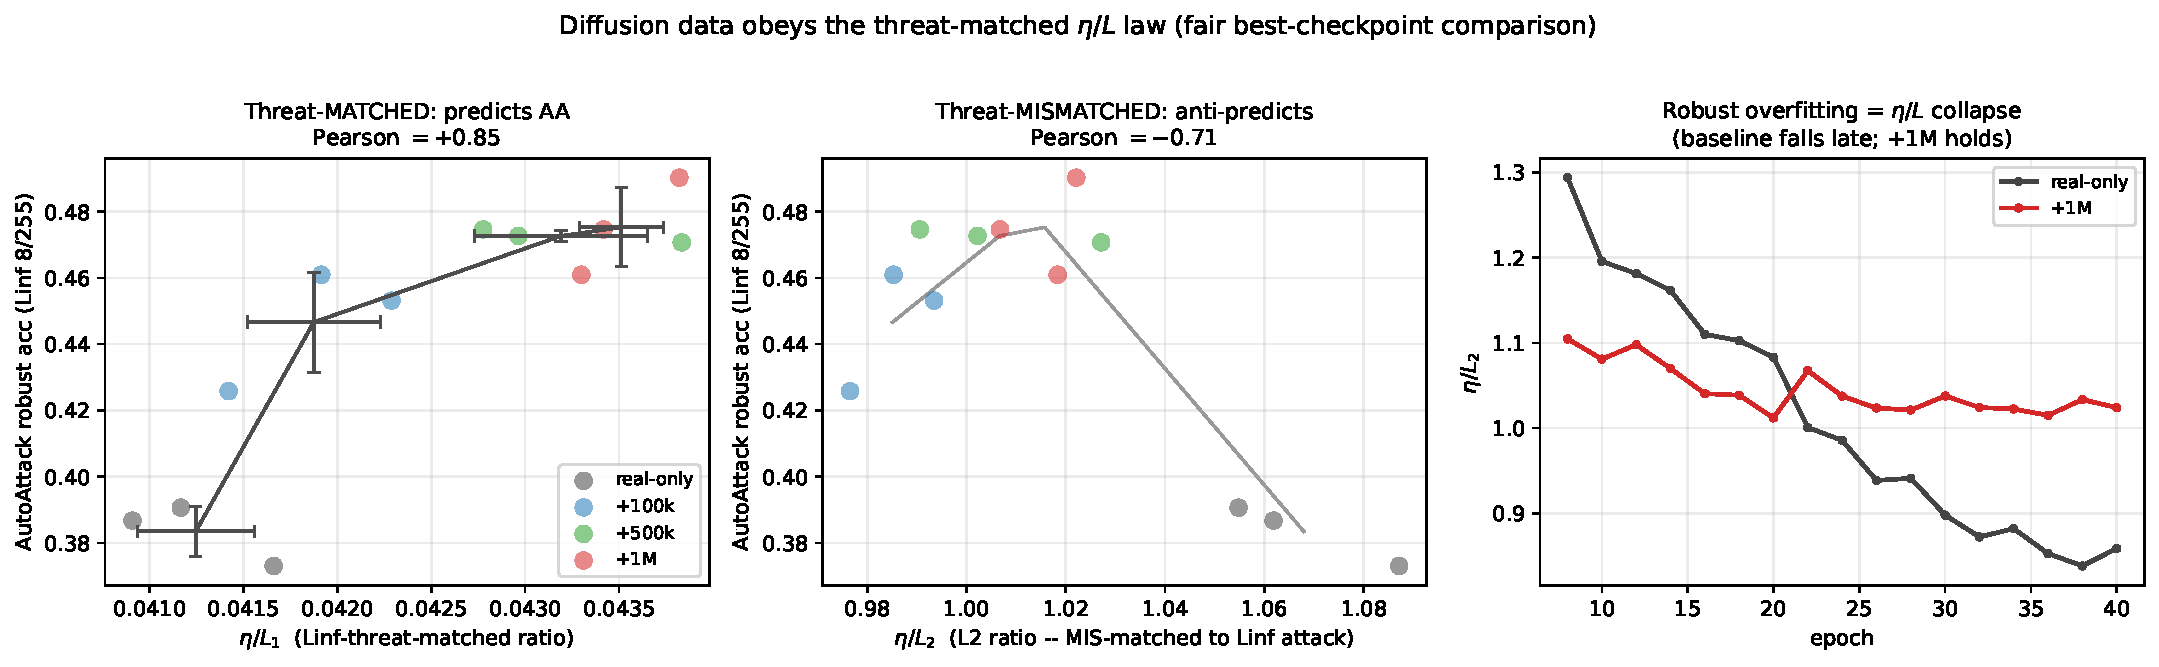
\includegraphics[width=\linewidth]{figures/diffusion_etaL_law.pdf}
\caption{Changing the data, not the architecture: diffusion-augmented adversarial training (CIFAR-10, $\ell_\infty{=}8/255$; four data doses, three seeds, best-robust checkpoints). Left: the threat-matched ratio $\eta/\|\nabla M\|_1$ tracks AutoAttack robust accuracy across the twelve dose-by-seed models (per-seed points faint, per-dose mean and standard deviation bold; Pearson $+0.85$). Middle: the mismatched $\ell_2$ ratio anti-predicts AutoAttack ($-0.71$); the real-only baseline has the highest $\ell_2$ ratio yet the lowest robustness. Right: over training, the real-only baseline's $\eta/L_2$ collapses as it robustly overfits while the $1$M-image model holds its value, so read through the ratio robust overfitting is an $\eta/L$ collapse the added data prevents.}
\label{fig:diffusion}
\end{figure}

\paragraph{The mechanism is dynamical, and coverage-gated.} The gain has a mechanism we can name and test. It is dynamical: synthetic data delays robust overfitting. Across the helping doses the robust-accuracy peak moves later (from epoch $19$ for real-only to $40$ for the augmented arms, Spearman $+0.94$ in synthetic amount; Figure~\ref{fig:mechanism}, left) and the late $\eta/L$ collapse the real-only baseline suffers (a drop of $0.48$ from its peak) is largely prevented (a drop of $0.06$ to $0.20$), so the model reaches a higher best-robust checkpoint before it memorizes the finite adversarial training set \citep{rice2020overfitting}. The gain also requires sufficient diversity. At a fixed real fraction, pools of $1$k or $10$k unique images give no gain (best-checkpoint AutoAttack $0.35$ to $0.38$, at or below the real-only $0.38$) while $100$k and above do ($0.45$ to $0.48$); this is a coverage threshold rather than a mixing artifact, because a $10$k pool still yields no gain when its synthetic batch share is reduced from seventy to thirty percent ($0.38$, essentially baseline) whereas $100$k helps at both shares ($0.44$ to $0.45$; Figure~\ref{fig:mechanism}, right). A too-small pool can additionally \emph{hurt} when over-mixed, the $10$k arm falling below baseline only at the seventy-percent share. The operative requirement for a gain is therefore sufficient vicinal coverage, for which Appendix~\ref{app:vicinal} gives a candidate static account, while the realized effect is the prevention of the dynamical $\eta/L$ collapse.

\begin{figure}[t]\centering
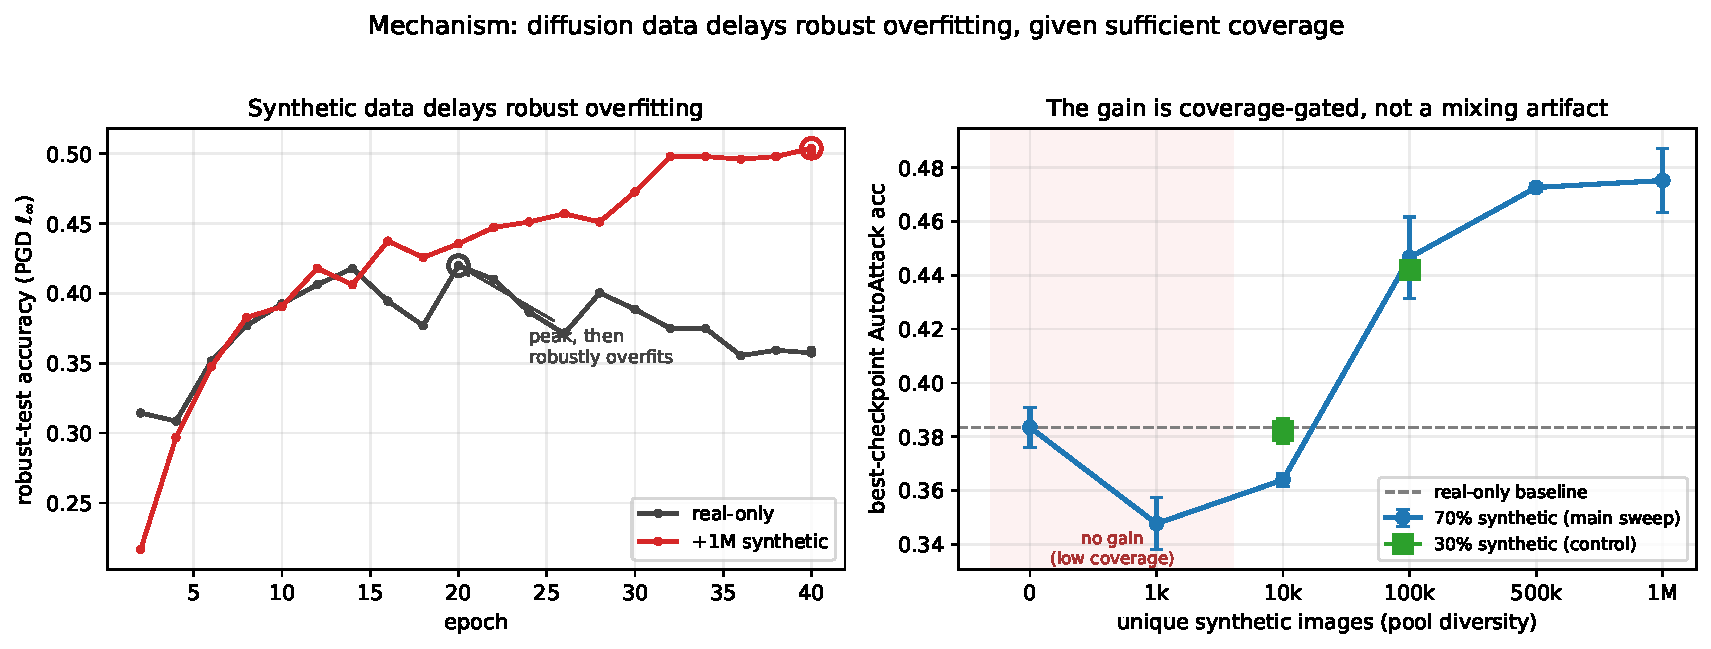
\includegraphics[width=\linewidth]{figures/diffusion_mechanism.pdf}
\caption{The data intervention works by delaying robust overfitting, given sufficient coverage. Left: robust-test accuracy over training (single seed, illustrative). The real-only model peaks near epoch $20$ and then robustly overfits, its robust accuracy decaying, while adding $1$M synthetic images postpones this so the model keeps improving. Right: best-checkpoint AutoAttack accuracy versus synthetic-pool diversity at the seventy-percent-synthetic mixing (three seeds), with the $10$k and $100$k control points at thirty-percent synthetic. Pools below about $100$k unique images give no gain at either mixing fraction, so the threshold is a coverage effect rather than an artifact of the mixing ratio.}
\label{fig:mechanism}
\end{figure}

\paragraph{The certificate holds per sample, not only across cells.} All the correlations so far, on both the architecture and the data axes, are between cell means. The same ratio also holds within a single model, sample by sample: read per input, the first-order ratio $M(x)/\|\nabla M(x)\|_2$ predicts that input's own minimum-norm (DDN) robust radius with Spearman $\rho\approx0.91$ under adversarial training and $\approx0.95$ under standard training, positive in every one of the thirty-six trained CIFAR-10 models (twelve standard, twenty-four adversarial) and $\approx0.97$ on CIFAR-100 (Figure~\ref{fig:persample}, left). The standard-training models are tighter because their smaller radii sit deeper in the locally linear regime where the first-order estimate is exact. This is the Lipschitz--margin certificate $r_2\gtrsim M/\|\nabla M\|_2$ \citep{hein2017formal,tsuzuku2018lipschitz} read pointwise; the first-order ratio is the small-curvature limit of the curvature-corrected bound of \citet{moosavi2019robustness}, and the input-gradient norm in its denominator is the dimension-dependent vulnerability of \citet{simongabriel2019first}. Its strong rank agreement with the exact minimum-norm attack quantifies how locally linear the models are and shows $\eta/L$ is a faithful per-sample robustness proxy, which is why the cell-mean correlation is so high.

\paragraph{Adversarial training inverts the within-model margin--sensitivity coupling.} A second per-sample observation concerns how a model trades margin against input sensitivity across its own inputs. Under standard training the within-model rank correlation between a sample's logit margin $M(x)$ and its input-gradient norm $\|\nabla M(x)\|_2$ is negative (Spearman $\approx-0.5$, all twelve standard-training models): high-margin points lie in flatter regions, so margin and robustness reinforce. Adversarial training flips the sign to positive ($\approx+0.5$, all twenty-four adversarially trained models; weaker on CIFAR-100), holding for the $\ell_1$ gradient norm as well and persisting when we restrict to the above-median-margin half (Figure~\ref{fig:persample}, right). We are not the first to relate logit margin to input sensitivity: that link is the Lipschitz--margin certificate, a margin consistency between logit and input-space margins has been documented in robust models \citep{ngnawe2024detecting}, and adversarial training is already known to reshape the input--loss geometry by reducing curvature \citep{moosavi2019robustness} and by aligning input gradients with semantic features \citep{tsipras2019robustness,ilyas2019adversarial}. What is specific here is the \emph{sign} of the per-sample coupling and its inversion: after adversarial training a model buys extra margin partly by raising local sensitivity, so the margin-to-sensitivity ratio is self-limiting, consistent with the modest robustness gains of forcing margin alone. Proposition~\ref{prop:split} gives the structural reason the coupling is positive and the ratio self-limiting: for a homogeneous network the radial floor $\|\nabla M(x)\|\ge M(x)/\|x\|$ forces larger margin to come with larger gradient.

\begin{figure}[t]\centering

\includegraphics[width=0.62\linewidth]{figures/resnet_persample_certificate.pdf}\hfill

\includegraphics[width=0.36\linewidth]{figures/resnet_persample_signflip.pdf}
\caption{Per-sample structure on the PreActResNet-18 models. Left: within one adversarially trained model, the first-order ratio $M/\|\nabla M\|_2$ predicts each point's own $\ell_2$ robust radius (Spearman $+0.91$); the right inset plots that within-model rank correlation for each model and it is positive in every one, across standard training, adversarial training, and CIFAR-100. Right: the within-model coupling between margin $M$ and input-gradient norm $\|\nabla M\|_2$ is negative under standard training and positive after adversarial training, for every model.}
\label{fig:persample}
\end{figure}

\paragraph{A practical reading: $\eta/L$ as an attack-free selection rule.} The dissection turns $\eta/L$ into a usable diagnostic for the common task of choosing which invariance operator to deploy for robustness. Computed from a trained model on clean inputs alone, as the mean active margin divided by the mean input-gradient norm, $\eta/L$ ranks the operators by their adversarial robust accuracy (Pearson $+0.93$ on the graded sweep, $+0.91$ on the ResNet backbone) without running any attack. We make this concrete as a selection rule. On each of five conditions (MNIST, Fashion-MNIST, and CIFAR-10 under $\ell_\infty$, CIFAR-10 under $\ell_2$, and a six-operator graded sweep), selecting the operator with the highest threat-matched $\eta/L$ picks the most robust operator in four conditions and the second best, within $0.3$ points, in the last: a mean AutoAttack regret of $0.06$ points against the oracle. Selecting by the highest shift-consistency instead picks a much worse operator, a mean regret of $8.8$ points of robust accuracy (up to $13$), because consistency is maximized by the exactly invariant operator, which is the least robust. Shift-consistency, the diagnostic the anti-aliasing literature foregrounds, is therefore the wrong signal for this choice. Clean accuracy is an equally good selector ($0.08$ points of regret), consistent with the margin being the common driver of \S\ref{sec:exp}; the operative point is the failure of consistency, not a margin of $\eta/L$ over clean accuracy. This is a selection rule, not a defense; whether $\eta/L$ can instead be a training objective is the question we turn to next.

\paragraph{$\eta/L$ is a diagnostic, not a trainable target.} A natural next step is to train $\eta/L$ directly. It does not work. On a standard backbone, four controlled interventions that penalize or maximize the ratio, namely an isotropic threat-matched gradient penalty, direct ratio maximization, an anisotropic hinge penalty, and a directional penalty at the adversarial point, each move $\eta/L$ at the diagnostic level but collapse the margin alongside it, leaving AutoAttack robust accuracy flat or worse with no gradient masking, as Proposition~\ref{prop:split} and Lemma~\ref{lem:ratiodegen} explain. Appendix~\ref{app:tmreg} reports the interventions in full.

\section{Related work}\label{sec:related}
\paragraph{The two regimes.} Whether shift-invariance helps or harms adversarial robustness has been argued in both directions. On the harming side, \citet{ge2021shift} prove that a fully shift-invariant classifier can be far less robust than a fully connected one. On the helping side, reducing aliasing has been shown to improve adversarial robustness in practice \citep{grabinski2022aliasing,grabinski2023fix,rodriguezmunoz2022aliasing}, and anti-aliased or learned-invariant pooling improves shift-consistency together with clean accuracy and corruption robustness \citep{zhang2019making,saha2024improving,michaeli2023alias}, and most recently \citet{wang2025bridging} build rotation- and scale-equivariant defenses and argue, through an orbit-invariant Lipschitz bound, that symmetry improves certified robustness. These findings have not been placed on a common axis; we do so through whether the discriminative signal is preserved under projection onto the invariant subspace with positive margin, summarized by $\eta/L$. A related trade-off line shows that geometric (spatial) invariance and adversarial robustness cannot both be maximized \citep{kamath2021canwehaveitall,tramer2019multiple}, and that more invariance raises vulnerability to invariance-based attacks \citep{tramer2020fundamental,gao2022limitations}; in our terms these are the small-$\eta/L$ and large-$\rho_G$ corners of the same criterion (\S\ref{sec:dich}).

\paragraph{What we add.} The Lipschitz--margin certificate $r_2\ge\eta/L$ is classical \citep{hein2017formal,tsuzuku2018lipschitz}, with deterministic \citep{leino2021globally} and randomized-smoothing \citep{cohen2019certified} descendants, and the per-sample link between logit margin and input-space margin has been documented in robust models \citep{ngnawe2024detecting}. Our contribution is not the bound but the shift-invariance dissection it supports: that shift-consistency does not predict robustness while a threat-matched $\eta/L$ does, and that adversarial training inverts the within-model margin--sensitivity coupling. The orbit-invariant Lipschitz mechanism of \citet{wang2025bridging} is, in this taxonomy, the shift-consistency ingredient we find necessary but not sufficient: our lazy-regime theorem (Appendix~\ref{app:bracket-lazy}) shares their observation that orbit-averaging is non-expansive, but shows that on orbit-complete data the invariant and unconstrained minimum-norm certificates coincide (so any advantage is a realized, finite-width effect, not a norm gap), adds the matching upper bound on the radius, and gives the margin-side account of the regime where invariance instead destroys the margin and hurts. On the optimization side, gradient descent provably converges to non-robust networks \citep{vardi2022gradient,frei2023double,li2025feature}, \citet{min2024can} conjecture an architectural fix, and \citet{melamed2023adversarial} tie non-robustness to off-manifold gradients; the neural-tangent-kernel account of robust versus non-robust features \citep{tsilivis2022what} underlies our lazy-regime result, and invariance has separately been used to aid robustness directly, for instance through test-time equivariance \citep{mao2023robust}. Architecture-versus-robustness studies \citep{huang2023revisiting} vary kernel, normalization, depth, and width under strong attacks but not shift-consistency. The robustness background is \citet{madry2018towards,goodfellow2015explaining,tsipras2019robustness}.

\section{Limitations and open problems}
The central open problem is a trajectory-level implicit-bias theorem for shift-invariant convolution-plus-pooling networks on data where the non-robustness premise genuinely holds (Proposition~\ref{prop:rank} shows the canonical orbit constructions are degenerate, while Proposition~\ref{prop:generic} shows generic orbit data is not, so such data exists). The criterion $\eta/L$ is a lower-bound certificate with no general converse, so the true robust radius can exceed it; the power-spectrum Lipschitz constant grows with input norm, so the guarantee is normalization-dependent; for real filters the convolution-square-pool layer spans conjugate-pair power coordinates rather than individual frequencies; the orbit-gradient statement is exact only for the continuous group; and the empirical study covers standard and PGD-adversarial training across three datasets (with a CIFAR-100 scaling check), two threat models, and small-convolutional and PreActResNet-18 backbones, so still larger architectures and the rich-regime trajectory analysis are left to future work. On the data axis, the mechanism we can verify is the prevention of a dynamical robust-overfitting $\eta/L$ collapse; the static vicinal-coverage account of Appendix~\ref{app:vicinal} is a falsifiable candidate for its coverage side rather than a confirmed generative mechanism, and the coverage threshold itself is characterized only empirically.

\bibliographystyle{plainnat}
\bibliography{references}

\appendix
\section{Proofs and additional results}\label{app:proofs}

\begin{proof}[Proof of Theorem~\ref{thm:A}]
Invariance of $g(x)=w^\top x+b$ under every shift means $w^\top S_s x=w^\top x$ for all $x,s$, i.e.\ $(S_{-s}w-w)^\top x=0$ for all $x$, so $S_{-s}w=w$ for all $s$; the only vectors fixed by every cyclic shift are the constants, hence $w\in\Vinv=\mathrm{span}(\mathbf 1)$. Writing $w=c\mathbf 1$, the score depends on $x$ only through $\fdc(x)=\mathbf 1^\top x/\sqrt\dd$, so the data reduce to the scalar DC values and the classes to the intervals $I_\pm$. The maximum-margin separator of two point sets on a line places the threshold midway between the nearer interval endpoints, with geometric margin half the distance between the intervals, giving $\gamma_{\mathrm{inv}}=\tfrac12\,\mathrm{dist}(I_+,I_-)$. Identifying the projected line with $\mathrm{span}(\mathbf 1)$ gives the convex-hull form.
\end{proof}

\begin{proof}[Proof of Proposition~\ref{thm:finite-group}]
$P_G$ is the orthogonal projector onto $V^G$: by group closure $P_G^2=|G|^{-2}\sum_{g,h}R_gR_h=|G|^{-1}\sum_k R_k=P_G$; each $R_g$ is orthogonal so $R_g^\top=R_{g^{-1}}$ and $P_G^\top=P_G$; its range is exactly the fixed subspace $V^G$. Invariance of $w^\top x$ for all $x$ is equivalent to $R_g^\top w=w$ for all $g$, hence (as $G$ is a group) to $R_g w=w$, i.e.\ $w\in V^G$. For $w\in V^G$ we have $w=P_Gw$, so $w^\top x=w^\top P_Gx$: every invariant linear classifier on $X_\pm$ is an ordinary linear classifier on the projected sets $P_GX_\pm$, with the same normal and signed margins. The maximum unit-normal margin separating two finite sets $A,B$ equals $\tfrac12\,\mathrm{dist}(\mathrm{conv}\,A,\mathrm{conv}\,B)$, attained by the unit vector along the closest-points segment of the hulls; applying this to $A=P_GX_+$, $B=P_GX_-$ gives the claim. The cyclic case has $P_G=\Pi_{\mathrm{inv}}$.
\end{proof}

\begin{proof}[Proof of Proposition~\ref{prop:rhoG}]
For any $h$ with $y_\star(R_hx)\neq y_\star(x)$, invariance gives $\mathrm{sign}\,g(R_hx)=\mathrm{sign}\,g(x)=y_\star(x)\neq y_\star(R_hx)$. Thus $R_hx$ is classified by $g$ as $y_\star(x)$ but the oracle label there is different, so $R_hx$ is an oracle-adversarial example at distance $\|R_hx-x\|_2$. Taking the infimum over such $h$ bounds the oracle-robust radius by $\rho_G(x)$.
\end{proof}

\begin{lemma}[Power-spectrum Lipschitz bound on a ball]\label{lem:ps-lip}
Let $Q(x)=(|\hat x_k|^2)_{k}$ with the unitary DFT. On $\|x\|_2\le B$, $\|Q(x)-Q(y)\|_2\le 2B\,\|x-y\|_2$, and a scalar quadratic invariant $f_a(x)=\sum_k a_k|\hat x_k|^2$ has $\|\nabla f_a(x)\|_2\le 2B\|a\|_\infty$.
\end{lemma}
\begin{proof}
For complex $z,z'$, $\big||z|^2-|z'|^2\big|\le|z-z'|\,(|z|+|z'|)$. Applying this coordinatewise to $Fx,Fy$ and using unitarity of $F$,
\[
\|Q(x)-Q(y)\|_2\le\|F(x-y)\|_2\big(\|Fx\|_2+\|Fy\|_2\big)=\|x-y\|_2\big(\|x\|_2+\|y\|_2\big)\le 2B\|x-y\|_2 .
\]
For the gradient, $\nabla f_a(x)=2F^{*}\mathrm{diag}(a)Fx$ in the real identification, so $\|\nabla f_a(x)\|_2\le 2\|a\|_\infty\|x\|_2\le 2B\|a\|_\infty$.
\end{proof}

\begin{proposition}[An exactly solvable nonlinear invariant model]\label{thm:toy}
Let $U,V$ be orthogonal subspaces of $\R^\dd$ and let $X_+=\{u\in U:\|u\|_2=a\}$, $X_-=\{v\in V:\|v\|_2=a\}$ (or finite shift-orbit subsets whose hulls contain $0$). The quadratic invariant $f(x)=\|P_Ux\|_2^2-\|P_Vx\|_2^2$ classifies $X_+,X_-$ correctly, every point has exact $\ell_2$ robust radius $a/\sqrt2$, and no linear classifier separates the classes.
\end{proposition}
\begin{proof}
For $x\in X_+$, $P_Vx=0$ and $\|x\|_2=a$, so $f(x)=a^2>0$. Decompose a perturbation as $\delta=\delta_U+\delta_V+\delta_W$ with $W=(U\oplus V)^\perp$. The boundary condition $f(x+\delta)\le0$ reads $\|x+\delta_U\|_2^2\le\|\delta_V\|_2^2$; $\delta_W$ cannot help, so set it to $0$. With $r=\|x+\delta_U\|_2$, the smallest $\|\delta_U\|_2$ is $|a-r|$ (move along the ray through $x$) and the smallest feasible $\|\delta_V\|_2$ is $r$, so $\|\delta\|_2^2\ge(a-r)^2+r^2$, minimized at $r=a/2$ with value $a^2/2$; hence the radius is $a/\sqrt2$, attained. The case $x\in X_-$ is symmetric. No affine hyperplane separates the classes because $0$ lies in both class convex hulls, so the hulls intersect.
\end{proof}

\begin{proof}[Proof of Proposition~\ref{prop:split}]
Degree-one homogeneity gives $M(x)=r\,m(u)$. For a perturbation $h=au+z$ with $z\perp u$, $D r(x)[h]=\langle u,h\rangle=a$ and $D u(x)[h]=z/r$ (tangent to the sphere), so $DM(x)[h]=a\,m(u)+\langle\nabla_{\mathbb S}m(u),z\rangle=\langle m(u)u+\nabla_{\mathbb S}m(u),\,h\rangle$ for all $h$; hence $\nabla M(x)=m(u)u+\nabla_{\mathbb S}m(u)$. Orthogonality gives the norm identity, and $m(u)=M(x)/\|x\|_2$ with $\nabla_{\mathbb S}\log m=\nabla_{\mathbb S}m/m$ gives the displayed form and the envelope equivalence.
\end{proof}

\begin{proof}[Proof of Lemma~\ref{lem:ratiodegen}]
Under $f\mapsto cf$ both $M$ and $\nabla M$ scale by $c$, leaving the ratio unchanged; the penalty $\mathbb E[\|\nabla M\|/M]\ge0$ attains its infimum $0$ only as $\nabla M\to0$, i.e.\ at a constant score, which classifies at chance. This is the constant-function degeneracy flagged by \citet{tsuzuku2018lipschitz}.
\end{proof}

\subsection{The two-sided bracket and the lazy-regime cluster theorem}\label{app:bracket-lazy}
We give in full the two results stated in the body: the conditional converse that completes the Lipschitz--margin certificate to a two-sided bracket (Proposition~\ref{prop:sandwich}, \S\ref{sec:dich}), and the lazy-regime cluster advantage that the optimization section invokes (\S\ref{sec:opt}).

\begin{proof}[Proof of Proposition~\ref{prop:sandwich}]
Write $y\in\{\pm1\}$ for the label of $x$, the margin $\eta:=y\,g(x)>0$, the decision
boundary $\mathcal B=\{z:g(z)=0\}$, and the robust radius
$r_2:=r_2(g,x)=\inf\{\|\delta\|_2:\mathrm{sign}\,g(x+\delta)\neq y\}$.
By hypothesis $g$ is continuous and $L$-Lipschitz in $\ell_2$ on a convex set $S$ that
contains $x$, the point of $\mathcal B$ nearest $x$, and the path $\gamma$ below;
convexity of $S$ keeps the relevant segments inside $S$, so the local Lipschitz and
co-Lipschitz constants apply along them.

\emph{Lower arm $r_2\ge\eta/L$.}
For any $\delta$ with $\|\delta\|_2<\eta/L$, the Lipschitz bound gives
$|g(x+\delta)-g(x)|\le L\|\delta\|_2<\eta=|g(x)|$, so $g(x+\delta)$ has the same sign as
$g(x)$ and $\mathrm{sign}\,g(x+\delta)=y$. No perturbation of norm below $\eta/L$ flips the
label, hence $r_2\ge\eta/L$ (the certificate of Corollary~\ref{cor:C};
\citealp{hein2017formal,tsuzuku2018lipschitz}).

\emph{Upper arm $r_2\le\eta/\alpha$.}
Let $\gamma:[0,T]\to S$ be a continuous path with $\gamma(0)=x$, $g(\gamma(T))=0$ (so $T$ is
the first time $\gamma$ meets $\mathcal B$), and a co-Lipschitz (lower-Lipschitz) bound
$|g(\gamma(t))-g(x)|\ge\alpha\|\gamma(t)-x\|_2$ holding up to $t=T$. Evaluating at $t=T$,
where $g(\gamma(T))=0$ and $|g(x)|=\eta$,
\[
\eta=|g(x)-g(\gamma(T))|\ \ge\ \alpha\,\|\gamma(T)-x\|_2,
\qquad\text{so}\qquad \|\gamma(T)-x\|_2\le \eta/\alpha .
\]
At $\gamma(T)\in\mathcal B$ we have $g(\gamma(T))=0$, so $\mathrm{sign}\,g(\gamma(T))\neq y$,
and by continuity of $g$ points immediately beyond $\gamma(T)$ have strictly opposite sign;
hence the perturbation $\delta=\gamma(T)-x$ is label-flipping and
$r_2\le\|\gamma(T)-x\|_2\le\eta/\alpha$.

\emph{$\alpha\le L$ and the condition number.}
Since $g(\gamma(T))=0\neq g(x)$ we have $\gamma(T)\neq x$, and the same secant obeys
$\alpha\|\gamma(T)-x\|_2\le|g(\gamma(T))-g(x)|\le L\|\gamma(T)-x\|_2$, so $\alpha\le L$ and
$\kappa:=L/\alpha\ge1$. Combining the two arms, $\eta/L\le r_2\le\eta/\alpha$, with
$r_2=\eta/L$ exactly when $\kappa=1$. The upper arm is informative only when $\alpha$ is
certified independently of $r_2$: taking $\alpha$ as the secant slope of the minimal path
itself makes $r_2=\eta/\alpha$ a tautology, whereas the linear case below and the
power-spectrum surrogate fix $\alpha$ from the feature structure, so the bracket is genuinely
two-sided there.

\emph{Linear (exact) case.}
If $g(x)=w^\top x+b$ is linear, in particular an invariant linear feature ($w\in\Vinv$, so
$g$ reads $x$ only through $\fdc$), then for every $z$,
$|g(z)-g(x)|=|w^\top(z-x)|\le\|w\|_2\|z-x\|_2$, with equality along the straight path
$\gamma(t)=x-t\,w/\|w\|_2$. Thus $L=\alpha=\|w\|_2$, $\kappa=1$, and the boundary is reached
at distance $\eta/\|w\|_2$, giving the exact point-to-hyperplane radius
$r_2=\eta/\|w\|_2$ \citep{hein2017formal}. The unbounded-$\kappa$ end is the
$t\mapsto t^{2n+1}$ feature of \S\ref{sec:dich} ($\eta/L=1/(2n+1)$ while $r_2=1$): no
universal converse exists, but every model sits in the bracket at its own finite or
infinite $\kappa$. The deterministic bracket complements the randomized-smoothing converse
of \citet{cohen2019certified}, whose looseness is a worst case over classifiers rather than
the explicit per-classifier $\kappa$ here.
\end{proof}

\begin{theorem}[Lazy-regime self-symmetrization: no minimum-norm certified-Lipschitz gap on orbit-complete data]\label{thm:lazy-cluster}
Work in the lazy/NTK regime, where each trained network equals the minimum-RKHS-norm
interpolant of its fixed neural tangent kernel \citep{jacot2018neural}: write
$K(x,x')=\langle\Phi(x),\Phi(x')\rangle_{\mathcal H}$ for the tangent kernel with feature
map $\Phi$ and RKHS $\mathcal H_K$, and assume a smooth activation so that $\Phi$ is
$L_\Phi$-Lipschitz on the data ball $\{\|x\|_2\le B\}$. Let the data be orbit-closed with
labels constant on orbits, let the kernel be shift-invariant
($K(S_sx,S_sx')=K(x,x')$ for all $s\in\Z_\dd$), and let
$\Pi_G f=\tfrac1\dd\sum_{s\in\Z_\dd}f(S_s\,\cdot)$ be the orbit-averaging (Reynolds)
operator, whose range $\mathcal H^G=\Pi_G\mathcal H_K$ is the invariant subspace realized by
the shift-tied orbit bundle of Lemma~\ref{lem:bundle}. For the unit-margin min-norm problem
$\min_{f}\|f\|_K$ s.t.\ $y_i f(x_i)\ge1$, let $f_{\mathrm{unc}}$ be the solution over
$\mathcal H_K$ and $f_{\mathrm{inv}}$ the solution over $\mathcal H^G$, and set the certified
Lipschitz constants $L_{\mathrm{unc}}=L_\Phi\|f_{\mathrm{unc}}\|_K$,
$L_{\mathrm{inv}}=L_\Phi\|f_{\mathrm{inv}}\|_K$. Then
\begin{enumerate}[leftmargin=1.7em,label=\textup{(\roman*)}]
\item $\Pi_G$ is the orthogonal projection of $\mathcal H_K$ onto $\mathcal H^G$, hence
  non-expansive, with $\|f\|_K^2=\|\Pi_G f\|_K^2+\|(I-\Pi_G)f\|_K^2$ \citep{elesedy2021provably};
\item $\Pi_G f_{\mathrm{unc}}$ is feasible for the invariant problem, so
  $\|f_{\mathrm{inv}}\|_K\le\|\Pi_G f_{\mathrm{unc}}\|_K\le\|f_{\mathrm{unc}}\|_K$;
\item therefore $L_{\mathrm{inv}}\le L_{\mathrm{unc}}$, and at the common unit margin $\eta$
  the invariant model has the weakly larger certified ratio,
  $\eta/L_{\mathrm{inv}}\ge\eta/L_{\mathrm{unc}}$. Moreover, because the RKHS norm is strictly
  convex and the data is orbit-closed, the unconstrained minimum-norm interpolant is itself
  invariant, $f_{\mathrm{unc}}=\Pi_G f_{\mathrm{unc}}$, so the orbit-variance
  $\|(I-\Pi_G)f_{\mathrm{unc}}\|_K^2$ vanishes and $L_{\mathrm{inv}}=L_{\mathrm{unc}}$: on
  orbit-complete data there is \emph{no} strict minimum-norm gap. A strict advantage requires
  non-orbit-complete data; the cluster-geometry advantage seen empirically is a
  realized-local-Lipschitz / finite-width effect, not a smaller min-norm certificate.
\end{enumerate}
\end{theorem}

\begin{proof}
(i) For a shift-invariant kernel, $\Pi_G$ is self-adjoint and idempotent on $\mathcal H_K$
with spectrum in $\{0,1\}$, hence the orthogonal projection onto its fixed-point set
$\mathcal H^G$; the displayed identity is the Pythagorean decomposition for that projection
\citep{elesedy2021provably}.
(ii) Because the data is orbit-closed with orbit-constant labels, each $S_s x_i$ is a
training point of label $y_i$, so $y_i f_{\mathrm{unc}}(S_s x_i)\ge1$ for all $s$, and
averaging gives $y_i(\Pi_G f_{\mathrm{unc}})(x_i)\ge1$. Thus $\Pi_G f_{\mathrm{unc}}\in
\mathcal H^G$ is feasible for the invariant min-norm problem, whence
$\|f_{\mathrm{inv}}\|_K\le\|\Pi_G f_{\mathrm{unc}}\|_K$, which (i) bounds above by
$\|f_{\mathrm{unc}}\|_K$.
(iii) For any $f\in\mathcal H_K$ and inputs $x,x'$ in the data ball,
$|f(x)-f(x')|=|\langle f,\Phi(x)-\Phi(x')\rangle_K|\le\|f\|_K\,\|\Phi(x)-\Phi(x')\|_K\le
L_\Phi\|f\|_K\,\|x-x'\|_2$, so $f$ is $L_\Phi\|f\|_K$-Lipschitz there. Applying this to
$f_{\mathrm{inv}}$ and $f_{\mathrm{unc}}$ and using (ii) gives $L_{\mathrm{inv}}\le
L_{\mathrm{unc}}$; dividing the common unit margin $\eta$ by these constants yields
$\eta/L_{\mathrm{inv}}\ge\eta/L_{\mathrm{unc}}$. The orthogonality identity of (i) makes the
norm gap exactly $\|(I-\Pi_G)f_{\mathrm{unc}}\|_K^2$. On orbit-complete data this gap is in fact
zero: each $S_s f_{\mathrm{unc}}$ is feasible (the orbit points are same-label training points)
with $\|S_s f_{\mathrm{unc}}\|_K=\|f_{\mathrm{unc}}\|_K$, so were $f_{\mathrm{unc}}$ non-invariant
the average $\tfrac1\dd\sum_s S_s f_{\mathrm{unc}}=\Pi_G f_{\mathrm{unc}}$ would be feasible of
strictly smaller norm by strict convexity, contradicting minimality; hence
$f_{\mathrm{unc}}=\Pi_G f_{\mathrm{unc}}$ and $L_{\mathrm{inv}}=L_{\mathrm{unc}}$.
\end{proof}

\begin{remark}[Reading and smooth-activation caveat]\label{rem:lazy-relu}
The norm contraction (i)--(ii) is activation-independent, but step (iii) uses smoothness:
the certified constant compared here is the RKHS-norm bound $L_\Phi\|f\|_K$ on the local
Lipschitz constant, not the realized constant. For a bare two-layer ReLU the tangent
feature map is not Lipschitz \citep{bietti2019inductive} (its RKHS contains unit-norm
functions of unbounded Lipschitz constant), so the theorem requires a smooth activation, or
an explicit $\sup_{\|x\|_2\le B}\|\nabla\Phi(x)\|$ bound carried in place of $L_\Phi$. The
result thus shows that in the lazy, smooth-activation regime the invariant and unconstrained
minimum-norm certificates coincide on orbit-complete data; the tied-versus-unconstrained
$\eta/L$ gap the synthetic stress test reports is therefore a realized, finite-width effect, and
the rich (small-init) and bare-ReLU trajectories, where the fixed-kernel picture breaks down
\citep{chizat2019lazy} and the realized-Lipschitz selection among equal-norm interpolants is the
open question, stay open.
\end{remark}

\begin{corollary}[Rich two-layer: the max-margin values coincide]\label{cor:no-gap-var}
The no-gap conclusion of Theorem~\ref{thm:lazy-cluster} needs only that the norm is $G$-invariant and convex and that Reynolds averaging preserves the orbit-constant margin constraints; the Hilbert-space projection is one instance. For any $G$-invariant convex norm $\|\cdot\|$, Jensen gives $\|\Pi_G f\|\le\int_G\|T_g f\|\,d\mu=\|f\|$, and on orbit-closed data $\Pi_G f$ is invariant and feasible, so the invariant and unconstrained unit-margin minimum-norm values coincide (strict convexity was used above only to conclude the unconstrained optimum is \emph{itself} invariant). In particular this holds for the variation (atomic) norm $\|f\|_{\mathcal V}=\inf_\rho\int|a|\,d|\rho|$ of an infinite-width two-layer network $f(x)=\int a\,\sigma(w^\top x)\,d\rho$ with an orthogonally $G$-closed activation dictionary. Since the directional limit of gradient descent on a homogeneous network is the minimum-variation-norm (max-margin) interpolant \citep{lyu2020gradient,ji2020directional}, weight sharing cannot raise that max-margin, which is the margin-free statement of \S\ref{sec:opt}. The variation norm is not strictly convex, so an invariant optimum exists but need not be unique; the open rich-regime question is therefore whether the dynamics select an invariant, lower-local-gradient optimum among equal-norm interpolants, not whether a smaller-norm optimum exists.
\end{corollary}

\subsection{The margin-gradient envelope at the implicit-bias solution}\label{app:envelope}
This backs the data-condition-number reading in \S\ref{sec:coupling}: the tangential factor of Proposition~\ref{prop:split} is bounded by the normalized margin the gradient-descent solution actually achieves, with no appeal to global optimality.
\begin{proposition}[Envelope via the achieved margin]\label{prop:ib-envelope}
Let $M_\theta(x_i)$ be the signed margin at $x_1,\dots,x_n\in\R^\dd\setminus\{0\}$, parameter-homogeneous of degree $p$ ($M_{a\theta}=a^pM_\theta$). Let $C$ satisfy $C(a\theta)=a^pC(\theta)$ and $\|\nabla_x M_\theta(x_i)\|_2\le B_iC(\theta)$ at differentiability points, and let the limiting gradient-descent direction $\bar\theta$ make $x\mapsto M_{\bar\theta}(x)$ positively $1$-homogeneous with $\min_iM_{\bar\theta}(x_i)>0$. With the achieved normalized margin $\gamma_{\mathrm{IB}}=\min_iM_{\bar\theta}(x_i)/C(\bar\theta)$ and the normalization $\widehat\theta=(\min_iM_{\bar\theta}(x_i))^{-1/p}\bar\theta$ (so $\min_iM_{\widehat\theta}(x_i)=1$), at every support point $M_{\widehat\theta}(x_i)=1$,
\[
\|\nabla_x M_{\widehat\theta}(x_i)\|_2\le\frac{B_i}{\gamma_{\mathrm{IB}}},\qquad
\|\nabla_{\mathbb S}\log m(u_i)\|_2\le\sqrt{\Big(\tfrac{B_i\|x_i\|_2}{\gamma_{\mathrm{IB}}}\Big)^2-1}.
\]
\end{proposition}
\begin{proof}
$\gamma_{\mathrm{IB}}$ is scale-invariant: $\bar\theta\mapsto a\bar\theta$ scales $\min_iM_{\bar\theta}(x_i)$ and $C(\bar\theta)$ both by $a^p$. With $\alpha=(\min_iM_{\bar\theta}(x_i))^{-1/p}$, parameter homogeneity gives $M_{\widehat\theta}(x_i)=\alpha^pM_{\bar\theta}(x_i)=M_{\bar\theta}(x_i)/\min_jM_{\bar\theta}(x_j)$, so $\min_iM_{\widehat\theta}(x_i)=1$, and $C(\widehat\theta)=\alpha^pC(\bar\theta)=C(\bar\theta)/\min_iM_{\bar\theta}(x_i)=1/\gamma_{\mathrm{IB}}$. The gradient-control hypothesis gives $\|\nabla_x M_{\widehat\theta}(x_i)\|_2\le B_iC(\widehat\theta)=B_i/\gamma_{\mathrm{IB}}$; dividing by $m(u_i)=M_{\widehat\theta}(x_i)/\|x_i\|_2$ in Proposition~\ref{prop:split} gives the spherical form.
\end{proof}
For a depth-$D$ bias-free network with $1$-Lipschitz $1$-homogeneous activations and $C(\theta)=(\|\theta\|_2/\sqrt D)^D$ the hypothesis holds with $B_i=\sqrt2$, since $\nabla_x M=J^\top(e_y-e_{j^\star})$ with $\|e_y-e_{j^\star}\|_2=\sqrt2$ and $\|J\|_2\le\prod_\ell\|W_\ell\|_2\le\prod_\ell\|W_\ell\|_F\le(\|\theta\|_2^2/D)^{D/2}=C(\theta)$ by the arithmetic--geometric-mean inequality. When the gradient-descent limit is globally max-margin, $\gamma_{\mathrm{IB}}$ is the global normalized margin and the bound is the global one; when it is only a KKT point \citep{lyu2020gradient,ji2020directional,vardi2022margin}, $\gamma_{\mathrm{IB}}$ is smaller and the bound weakens, as it must. The constant cannot be data-independent: for $(\pm e_1,\pm1),(\pm e_2/A,\pm1)$ in $\R^2$ the hard-margin solution is $w^\star=(1,A)$, giving $\|\nabla_{\mathbb S}\log m(e_1)\|_2=A\to\infty$; the linear case is exact with $\tau_i=\|x_i\|_2/\gamma$ \citep{soudry2018implicit}.

\subsection{Per-arm robust accuracies under adversarial training}\label{app:at-tables}
Table~\ref{tab:at-general} reports the correlations that summarize the generality experiment of \S\ref{sec:exp}; Table~\ref{tab:at-perarm} gives the per-arm AutoAttack robust accuracies behind them, with clean accuracy and circular-shift consistency alongside. The numbers make the saturation on MNIST explicit: at $\ell_\infty=0.3$ every arm is robust to within one point of $94\%$, so the across-arm spread that the consistency correlation reads is narrow, which is why that correlation, though still negative, is not significant at this grid size. On Fashion-MNIST and $\ell_2$-CIFAR the spread is several times wider and the exactly invariant arm, whose consistency is $1.0$ by construction, is the least robust in each width.

\begin{table}[h]\centering
\caption{Per-arm AutoAttack robust accuracy under PGD adversarial training for the three generality conditions (means over two seeds). MNIST and Fashion-MNIST are $\ell_\infty$-trained and evaluated at the listed threshold; CIFAR-10 is $\ell_2$-trained and evaluated at $\ell_2=0.5$. Clean accuracy and circular-shift consistency are shown for reference. The four arms share a channel schedule and so an identical parameter count at each width.}
\label{tab:at-perarm}
\small
\begin{tabular}{ll ccc}
\toprule
arm & $w$ & clean & consist. & robust acc. \\
\midrule
\multicolumn{5}{l}{\emph{MNIST}, $\ell_\infty=0.3$} \\
standard & 32 & 0.994 & 0.945 & 0.942 \\
anti-aliased & 32 & 0.994 & 0.953 & 0.942 \\
exact cyclic & 32 & 0.994 & 1.000 & 0.926 \\
shift-aug & 32 & 0.994 & 0.998 & 0.939 \\
standard & 64 & 0.994 & 0.946 & 0.947 \\
anti-aliased & 64 & 0.994 & 0.954 & 0.947 \\
exact cyclic & 64 & 0.994 & 1.000 & 0.934 \\
shift-aug & 64 & 0.995 & 0.999 & 0.952 \\
\midrule
\multicolumn{5}{l}{\emph{Fashion-MNIST}, $\ell_\infty=0.1$} \\
standard & 32 & 0.876 & 0.684 & 0.776 \\
anti-aliased & 32 & 0.876 & 0.683 & 0.776 \\
exact cyclic & 32 & 0.855 & 1.000 & 0.724 \\
shift-aug & 32 & 0.862 & 0.958 & 0.747 \\
standard & 64 & 0.886 & 0.680 & 0.781 \\
anti-aliased & 64 & 0.885 & 0.690 & 0.783 \\
exact cyclic & 64 & 0.868 & 1.000 & 0.736 \\
shift-aug & 64 & 0.870 & 0.964 & 0.760 \\
\midrule
\multicolumn{5}{l}{\emph{CIFAR-10}, $\ell_2=0.5$} \\
standard & 32 & 0.804 & 0.829 & 0.581 \\
anti-aliased & 32 & 0.815 & 0.832 & 0.594 \\
exact cyclic & 32 & 0.711 & 1.000 & 0.464 \\
shift-aug & 32 & 0.794 & 0.902 & 0.570 \\
standard & 64 & 0.846 & 0.847 & 0.609 \\
anti-aliased & 64 & 0.854 & 0.857 & 0.628 \\
exact cyclic & 64 & 0.769 & 1.000 & 0.511 \\
shift-aug & 64 & 0.841 & 0.924 & 0.613 \\
\bottomrule
\end{tabular}
\end{table}

\subsection{Four interventions confirm $\eta/L$ is not a trainable target}\label{app:tmreg}
The scale-invariance of Lemma~\ref{lem:ratiodegen} makes the ratio objective degenerate, and the radial floor of Proposition~\ref{prop:split} ties the gradient to the margin; whether a first-order penalty can nonetheless raise $\eta/L$ into robustness is then an empirical question, which we settle with four controlled interventions on a standard backbone. \emph{(1)~Isotropic gradient penalty.} Adding to adversarial training a penalty on the threat-matched margin gradient $\|\nabla M\|_1$, the quantity the criterion is built on, against three controls (vanilla adversarial training, the $\ell_2$ loss-gradient penalty of \citet{ross2018improving,finlay2021scaleable}, and the same margin penalty with the mismatched $\ell_2$ norm; two widths, two seeds, Figure~\ref{fig:tmreg}) does at the diagnostic level exactly what the criterion predicts: only the threat-matched $\ell_1$ penalty raises $\eta/L$ (the input-gradient $\ell_1$ norm falls from $38$ to $22$ as the penalty strengthens), while the mismatched $\ell_2$ and loss-gradient penalties leave it unchanged. The higher $\eta/L$ does not translate into robustness: AutoAttack robust accuracy is statistically unchanged for every moderate penalty (paired $p>0.4$ against adversarial training) and falls under the strongest matched penalty ($-0.011$, $p=0.026$), with no gradient masking, because penalizing the gradient lowers the margin alongside it ($\eta$ falls from $1.58$ to $1.03$), so the higher $\eta/L$ buys nothing. \emph{(2)~Ratio maximization.} Penalizing the margin-normalized sensitivity $\|\nabla M\|_1/M$ directly drives the classifier to the trivial constant solution, with margin and sensitivity both vanishing and accuracy at chance, the scale-invariance degeneracy of Lemma~\ref{lem:ratiodegen}. \emph{(3)~Anisotropic hinge penalty} (a hinge-to-target on the margin gradient) and \emph{(4)~directional penalty} at the adversarial point (two widths, two seeds, $30$ epochs) reach for the same decoupling through anisotropic and input-direction-aware penalties, and collapse in the same way: clean accuracy falls from $0.728$ to $0.38$ and $0.30$, AutoAttack robust accuracy from $0.390$ to $0.258$ and $0.201$, and the margin from $1.59$ to $0.24$ and $0.05$, every quantity dropping together with no gradient masking. All four interventions collapse the margin: $\eta/L$ is a faithful cross-model diagnostic but not a trainable objective. The scale-invariance degeneracy (Lemma~\ref{lem:ratiodegen}) and the radial floor (Proposition~\ref{prop:split}, whose tangential slack is large at the operating point) are the structural backdrop; the collapse itself is an empirical regularity across all four penalty designs.

\begin{figure}[t]\centering
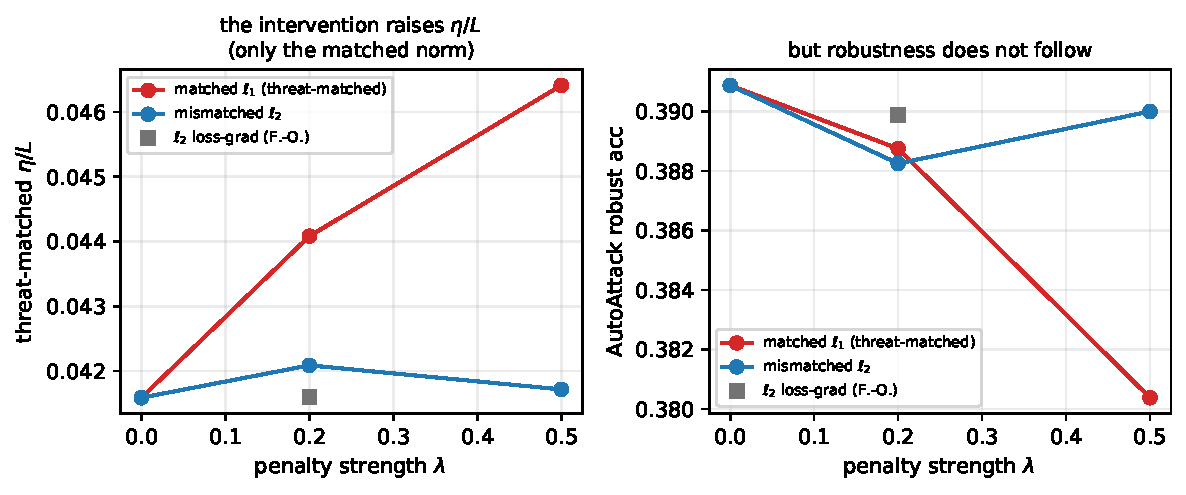
\includegraphics[width=0.84\linewidth]{figures/tmreg.pdf}
\caption{Regularizing $\eta/L$ during adversarial training (standard backbone; means over widths and seeds). Left: only the threat-matched $\ell_1$ margin penalty raises $\eta/L$ as its strength $\lambda$ grows; the mismatched $\ell_2$ margin penalty and the $\ell_2$ loss-gradient penalty leave it flat. Right: the higher $\eta/L$ does not raise AutoAttack robust accuracy, which is flat and then falls. Raising $\eta/L$ by penalizing the gradient also shrinks the margin (the self-limiting coupling), so $\eta/L$ is a diagnostic, not a trainable target.}
\label{fig:tmreg}
\end{figure}

\subsection{A candidate static mechanism: vicinal gradient coverage}\label{app:vicinal}
We report the data-intervention result of \S\ref{sec:exp} at the level of the diagnostic, $\eta/L$ rises and predicts robustness, without committing to a generative mechanism, because the network-level effect we can verify is dynamical: the added data prevents the robust-overfitting collapse of $\eta/L$ rather than producing a smoother solution at matched robustness. This appendix records a \emph{candidate static} mechanism that is consistent with the gauge-invariant observations and makes falsifiable predictions we test. It is a hypothesis about how synthetic gradient coverage could lower the realized sensitivity, not a claim that the trained network optimizes this objective.

\paragraph{First-order adversarial training is input-gradient regularization.}
\begin{lemma}[First-order robust-loss expansion]\label{lem:first-order-at}
Let $\ell:\R^d\to\R$ be twice continuously differentiable on $B_\varepsilon(x)=\{x+\delta:\|\delta\|\le\varepsilon\}$ for a norm $\|\cdot\|$ with dual $\|\cdot\|_*$, with $\|\nabla^2\ell(z)\|_{\mathrm{op}}\le H$ on $B_\varepsilon(x)$. Then
\[ \sup_{\|\delta\|\le\varepsilon}\ell(x+\delta)=\ell(x)+\varepsilon\|\nabla\ell(x)\|_*+R_\varepsilon(x),\qquad |R_\varepsilon(x)|\le\tfrac H2\varepsilon^2 . \]
\end{lemma}
\begin{proof}
Set $g=\nabla\ell(x)$. Taylor with remainder gives $\ell(x+\delta)=\ell(x)+\langle g,\delta\rangle+\tfrac12\delta^\top\nabla^2\ell(x+s\delta)\delta$ for some $s\in[0,1]$, and the quadratic term is at most $\tfrac H2\varepsilon^2$ in magnitude. With $\langle g,\delta\rangle\le\|g\|_*\varepsilon$ the supremum is at most $\ell(x)+\varepsilon\|g\|_*+\tfrac H2\varepsilon^2$; choosing $\delta=\varepsilon v$ with $\|v\|\le1$ and $\langle g,v\rangle=\|g\|_*$ gives the matching lower bound.
\end{proof}
If $\ell(x,y)=\phi(M(x,y))$ then $\nabla_x\ell=\phi'(M)\nabla_xM$, so on a margin band where $|\phi'|$ is bounded away from $0$ and $\infty$ the first-order penalty controls the sensitivity $L=\mathbb{E}\|\nabla_xM\|$ that enters the radius proxy.

\paragraph{The vicinal gradient-coverage matrix.}
Linearize the margin in parameters, $M_\theta(x)=\theta^\top\psi(x)$ with $J_\psi(x)=\nabla_x\psi(x)$, so $\nabla_xM_\theta(x)=J_\psi(x)^\top\theta$ and $\|\nabla_xM_\theta(x)\|_2^2=\theta^\top J_\psi(x)J_\psi(x)^\top\theta$. For a (data or vicinal) measure $\nu$ define the gradient-coverage matrix $Q_\nu:=\int J_\psi J_\psi^\top\,d\nu$, so $\int\|\nabla_xM_\theta\|_2^2\,d\nu=\theta^\top Q_\nu\theta\ge0$. Adding synthetic data changes $\nu$, adding a positive-semidefinite $Q_{\mathrm{syn}}$ to the input-gradient penalty.

\begin{theorem}[Synthetic coverage filters high-sensitivity modes]\label{thm:vic-filter}
Let $A\succ0$, $Q\succeq0$ be symmetric, $a\in\R^p$; for $t\ge0$ set $B_t=A+tQ$, $\theta_t=B_t^{-1}a$, $\eta(t)=a^\top\theta_t$, $S(t)=\theta_t^\top Q\theta_t$. Then $\eta'(t)=-S(t)\le0$ and $S'(t)=-2\theta_t^\top QB_t^{-1}Q\theta_t\le0$.
\end{theorem}
\begin{proof}
$\theta_t=B_t^{-1}a$ minimizes the strictly convex $\tfrac12\theta^\top B_t\theta-a^\top\theta$. Differentiating $B_t\theta_t=a$ with $B_t'=Q$ gives $\theta_t'=-B_t^{-1}Q\theta_t$. Then $\eta'(t)=a^\top\theta_t'=\theta_t^\top B_t\theta_t'=-\theta_t^\top Q\theta_t=-S(t)$, and $S'(t)=2\theta_t'^\top Q\theta_t=-2\theta_t^\top QB_t^{-1}Q\theta_t\le0$ since $B_t^{-1}\succ0$.
\end{proof}

\begin{theorem}[Two-mode model: the ratio rises iff a smooth mode remains]\label{thm:vic-twomode}
Let $\theta=(\theta_s,\theta_r)$, $A=I_2$, $Q=\begin{psmallmatrix}0&0\\0&q\end{psmallmatrix}$ with $q>0$, and $a=(a_s,a_r)$ with $a_r\neq0$. With $\eta(t)=a^\top\theta_t$, the root-mean-square sensitivity $L(t)=\sqrt{\theta_t^\top Q\theta_t}$ (the $L^2(\nu)$ analogue of the mean $L=\mathbb E\|\nabla M\|$ of the body; the gauge argument is identical for either), and $\rho(t)=\eta(t)/L(t)$,
\[ \theta_t=\Big(a_s,\tfrac{a_r}{1+tq}\Big),\quad \eta(t)=a_s^2+\tfrac{a_r^2}{1+tq},\quad L(t)=\tfrac{\sqrt q\,|a_r|}{1+tq},\quad \rho(t)=\tfrac{(1+tq)a_s^2+a_r^2}{\sqrt q\,|a_r|}, \]
and $\eta'(t)<0$, $L'(t)<0$, $\rho'(t)=\sqrt q\,a_s^2/|a_r|>0$ iff $a_s\neq0$. Both $\eta$ and $L$ fall, $L$ faster, and the ratio rises exactly when a smooth low-sensitivity mode remains.
\end{theorem}
\begin{proof}
$(I_2+tQ)=\operatorname{diag}(1,1+tq)$ gives $\theta_t$ and $\eta(t)$ directly; $Q\theta_t=(0,qa_r/(1+tq))^\top$ gives $L(t)=\sqrt q|a_r|/(1+tq)$. Differentiating, $\eta'(t)=-qa_r^2/(1+tq)^2<0$ and $L'(t)=-q\sqrt q|a_r|/(1+tq)^2<0$; the numerator of $\rho$ has $t$-derivative $qa_s^2$ over a constant denominator, so $\rho'(t)=\sqrt q\,a_s^2/|a_r|$, positive iff $a_s\neq0$.
\end{proof}

\begin{remark}[Gauge status of the decomposition]\label{rem:vic-gauge}
The map $\theta\mapsto c\theta$ scales $\eta\mapsto c\eta$ and $L\mapsto cL$, so $\rho=\eta/L$ is invariant while $\eta$ and $L$ individually are not; a trained network has exactly this freedom (Lemma~\ref{lem:ratiodegen}). The separate signs $\eta'(t)<0$ and $L'(t)<0$ are stated in the $A=I$ (weight-norm) gauge, which corresponds to the logit-norm anchor of \S\ref{sec:exp}: under that anchor the multi-seed run reproduces ``$\eta$ falls, $L$ falls faster'', while under a temperature anchor the split reverses. Only $\rho'(t)>0$ is anchor-free.
\end{remark}

\begin{corollary}[Pure-temperature degeneracy]\label{cor:vic-temp}
If $a_s=0$ then $\rho(t)=|a_r|/\sqrt q$ is constant: suppressing a single rough margin-carrying mode scales $\eta$ and $L$ together and cannot raise the ratio. A genuine gain requires a remaining smooth component $a_s\neq0$.
\end{corollary}
\begin{proof}
Set $a_s=0$: $\rho(t)=a_r^2/(\sqrt q|a_r|)=|a_r|/\sqrt q$, independent of $t$.
\end{proof}

\begin{corollary}[Uniform gradient-shape shrinkage]\label{cor:vic-shape}
If the gradient field is dominated by the rough mode, $\nabla_xM_{\theta_t}\approx\theta_{r,t}g_r$ with $g_r$ independent of $t$, then for any two homogeneous norms $\|\cdot\|_\alpha,\|\cdot\|_\beta$ the ratio $\|\nabla_xM_{\theta_t}\|_\alpha/\|\nabla_xM_{\theta_t}\|_\beta\approx\|g_r\|_\alpha/\|g_r\|_\beta$ is approximately independent of $t$: $L_1$ and $L_2$ can both fall sharply while $L_1/L_2$ stays nearly constant.
\end{corollary}

\paragraph{What this does and does not establish.} The model is a local linearization at a fixed gauge. Its \emph{gauge-free} predictions hold in our experiments: $\eta/L$ rises (it crosses $1$ and saturates), $L_1/L_2$ stays nearly constant while both norms fall (from about $25.5$ to $23.6$), and the largest sensitivity drop occurs on vicinal and interpolation points, which a manifold probe confirms. Its decomposition narrative does not survive a full analysis: the ``$\eta$ falls, $L$ falls faster'' reading is gauge-relative (Remark~\ref{rem:vic-gauge}), and at the matched best-robust checkpoint the realized $L$ is not in fact lower (\S\ref{sec:exp}). The operative network-level effect is therefore robust-overfitting prevention, of which this static path result is at most the coverage-side ingredient; we record it as a falsifiable hypothesis, not as the confirmed mechanism.

\end{document}
